 \documentclass[letterpaper,10pt]{article}
\usepackage{amsmath}
\usepackage[utf8x]{inputenc}
\usepackage{caption}
\usepackage{subcaption}
\usepackage{graphicx}
\usepackage{subfig}
\usepackage{float}
\usepackage{natbib}
\usepackage{anysize}
\usepackage{float}
\usepackage{tabularx}
\usepackage{amsmath}
\DeclareMathOperator{\sgn}{sgn}
\usepackage{amssymb}
\usepackage{amsfonts}
\usepackage{mathrsfs}
\usepackage{setspace}
\usepackage{relsize}
\usepackage{color}
\usepackage{multicol}
\newcommand{\red}[1]{\textcolor{red}{#1}}
%
%\marginsize{1.in}{1.in}{1in}{1in}
%\linespread{1.25}
%\setlength\parindent{0pt}
\title{Heuristic and Eulerian Interface Capturing Approaches for Shallow Water Type Flow and Application to Granular Flows }
\author{Hossein Aghakhani, Keith Dalbey, Abani Patra, David Salac}
\date{}
\begin{document}
\maketitle
\begin {abstract}{
Determining the wet-dry boundary and the related spurious thin-layer problem has historically been a challenge when 
solving the depth-averaged shallow-water (SW) equations (or similar granular flow's equations), and has 
been the focus of much research effort. In this paper we introduce the use of level set and phase field based methods to solve this issue and related problems. We also propose new heuristic 
methods to address this problem. We implemented all of these methods in TITAN2D, which is a parallel adaptive mesh refinement toolkit designed for numerical simulation of granular flows. 
Results of the methods for flow over a simple inclined plane and Colima volcano are used to illustrate the methods. For the inclined plane we verified the results with experimental data and for 
Colima volcano they have been compared with field data. We successfully captured the interface of the flow and solved the accuracy and stability problems related to the thin layer problem in 
SW numerical solution. The comparison of results shows that although all of the methods can be used to address this problem, 
each of them has its own advantages/disadvantages and methods have to be chosen carefully for each problem.
\textbf{Keywords:} Shallow water flow, Thin layer, Wetting/Drying, Phase field, Level set}
\end{abstract}
% =============================================================================
%                 INTRODUCTION
% =============================================================================
\section{Introduction} 
\label{introduction}
% Basic introduction about the Shallow water
%%{\bf NEED MORE CITATIONS}
Shallow water (SW) flows include a wide range of fluid flows. In SW flows the fluid depth is much 
smaller (${\cal O}(10^{-1})$) than the characteristic length of the fluid body. In deriving the corresponding 
governing equations the shallowness of flow allows us to approximate the variation of state variables in the direction perpendicular to the basal surface and replace
them with an integrated average \cite{SavageHutter}, which
reduces a three dimension flow into a two-dimensional problem.
This approximation holds for many circumstances in geophysical flows and the same 
conservation equations with some minor variations can be used to study varying physical situations.
Eglit and Sveshnikova \cite{eglit1980mms} modified the depth-averaged Saint Venant equations to simulate granular snow avalanches and almost a decade later 
Savage and Hutter \cite{SavageHutter} popularized these in the modeling of many geophysical mass flows related to landslides, avalanches and debris flows. 
% introducing WD problem
Since this type of flow has free moving boundaries one of the basic difficulties 
of the numerical solution is identifying the location of flow interface. 
Furthermore, the governing equations are valid only in the wet areas so we need an strategy to discriminate between wet and dry areas in the numerical simulation. 
In the SW context this is usually called the {\it wetting and drying (WD)} problem. %or {\it thin-Layer} problem 
In our previous work, see Ref. \cite{Patra2005}, we showed how the speed of waves has to be modified for flow near the vacuum region based on Toro \cite{ToroBook2001} to mitigate 
the stability problem. However, this still leads to the formation of a non-physical thin layer in the numerical solution, see figure \ref{thinlayerproblem} for an illustration.
This non-physical thin layer could extend large distances from the realistic main 
body of the flow, which can cause inaccurate construction of the boundary, loss of conservation or severe 
numerical instabilities in the numerical solution. 
Beside the numerical issues, determining probable flow extents through numerical simulation is critical for many SW problems, especially for geophysical flow. For example, in preparing a hazard map 
for a volcano or a flood it is crucial to know the location of the front of the flow to answer basic questions such as --  Does the flow reach a specific location? What is the distance of high 
risk locations from civil infrastructure? 
The answer of all the above questions is not possible without good information about the interface of the flow along its flow path.
\begin{figure}[t]
  \begin{minipage}[b]{.45\linewidth}
    \centering
    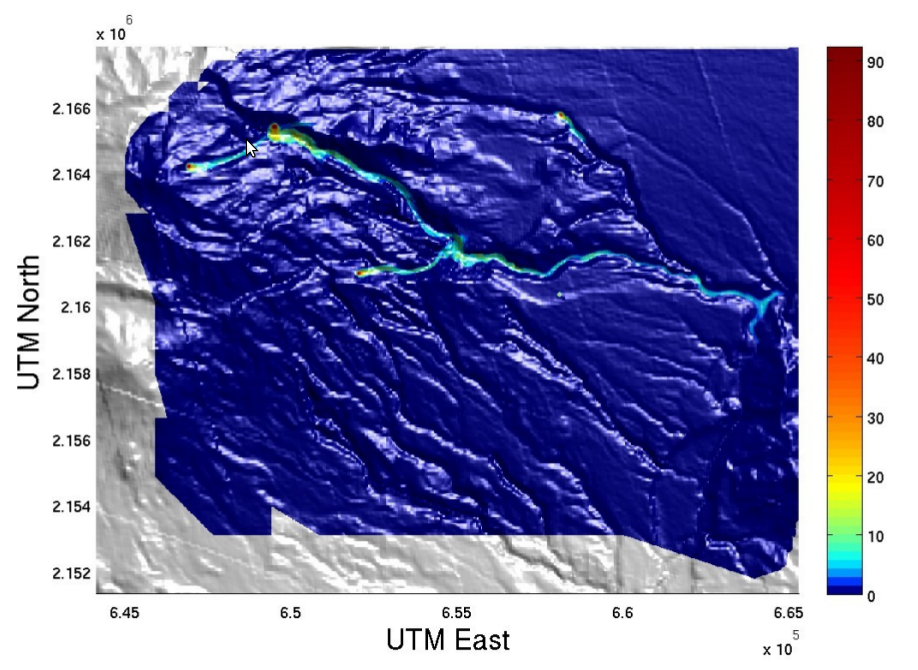
\includegraphics[width=1\textwidth]{IMAGES/rupps1.png}
    \subcaption{ Without thin layer control}
  \end{minipage}
\hspace{0.5cm}
%   \hfill
  \begin{minipage}[b]{.45\linewidth}
    \centering
    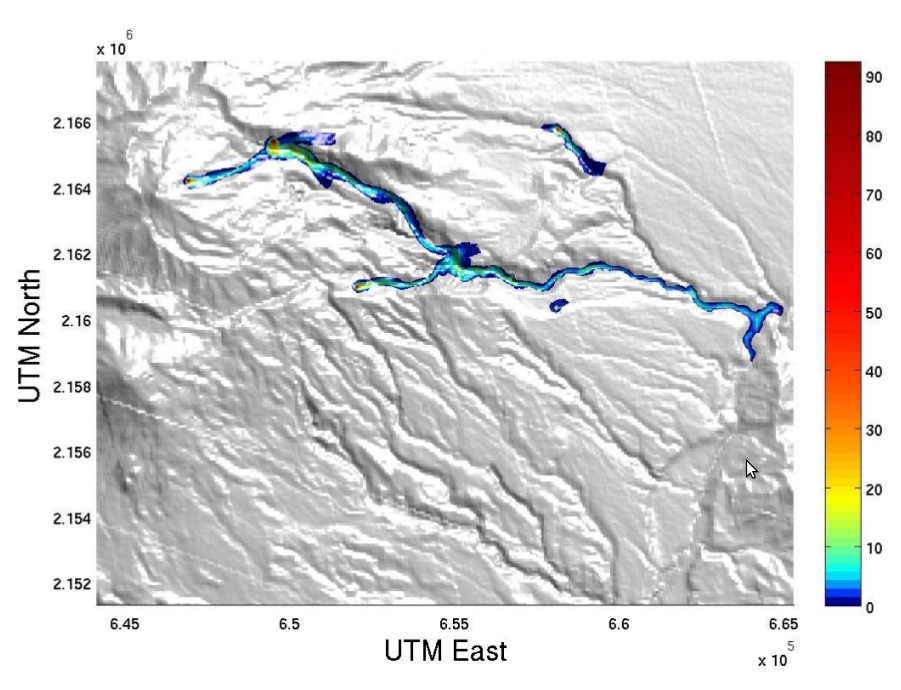
\includegraphics[width=1\textwidth]{IMAGES/rupps2.png}
    \subcaption{Only flow with depth greater than 0.5 m is displayed.}
   \end{minipage}
  \caption{Thin layer problem in maximum over time flow depth simulation of the 1955 debris flow at Atenquique, Mexico \cite{Dalbey2009}.}
  \label{thinlayerproblem}
\end{figure}
A demonstration of possible issues in shown in Figure \ref{thinlayerproblem}.
In this figure the numerical simulation of block and ash flows in Atenquique, which is a village near the Colima volcano in Mexico, using a SW like model 
based on a granular flow assumption is shown. The left figure shows the numerical solution of flow height without using any control for the thin layer problem 
and the right figure shows the same result  
using a naive control -- plotting the regions with flow height $h>0.5m$. If no heuristic control on the numerical solution is used the thin layer causes instability and 
inaccuracy in the obtained results.
To summarize, the following major difficulties arise in numerical solutions of SW flows related to the WD or thin layer problem:
\begin{enumerate}
        \item Ambiguous and subjective computation of flow spreads in SW flows.
        \item \label{problemwicking}
             Unphysically fast estimate of the flow speed. As the solution of SW equations are momentum, $\{hV_x,hV_y\}$, to find velocities, $\{V_x,V_y\}$, used during the solution process the
             momentum must be divided by flow depth, $h$, which causes a numerical error if $h$ is small and results in overly large velocities.
        \item \label{problemtoothin}
              Unphysical thin layer (orders of magnitude thinner than a grain of sand). This results from the combination of conservation of mass and the numerical wicking away of material.
        \item \label{problemunstable}
              Loss of numerical stability. Due to the above reasons wave-speeds can become infinite at the flow boundary which means that flow equations lose their hyperbolicity  
              at the vacuum state interface.
\end{enumerate}\label{thinprob}
\subsection{Background and Review}
A review of the literature shows numerous attempts have been made to overcome these problems \cite{Medeiros2013,Balzano1998,Aureli2008,Bunya2009,Casulli2009a,
Kesserwani2011,DAlpaos2007,Castro2005}.
Here we briefly review the problem and recent approaches and refer the interested reader to available references for more information.
Generally, all of the approaches can be 
categorized into two basic groups which we call heuristic methods and interface tracking/capturing methods.
The basic idea of heuristic methods is to reconstruct the flow interface based upon 
some simple heuristic or some algebraic relations. In this approach, the reconstruction could take into account the physics of the problem, but this is not required. 
For example, to mitigate the thin layer problem a threshold could be defined to control the thin layer, the entire domain could be filled with a shallow level of fluid,
the flow could be recontructed, or the flux could be adjusted. It is possible to use any combination of these heuristic fixes.
Most of attempts that are made to address the thin layer problem are categorized under this sort of method \cite{Aureli2008,Bunya2009,Castro2005,Kesserwani2011}.
In interface tracking/capturing approaches
an auxiliary set of equations is coupled to the original problem. This auxiliary set of equations is used to follow the flow interface over time. 
Unlike hueuristic method in interface tracking/capturing methods one can find the interface of a moving boundary flow in a more rigorous way. 
The particular choice of the auxilary equations leads to either interface tracking, or Lagrangian, methods or interface capturing, or Eulerian, methods.
In Lagrangian methods the front is replaced with a set of interfacial points which explicitly define the location of the interface.
During each time step these points move due to the numerically computed velocity field.
Mark And Cell (MAC) \cite{Harlow1965}, Simplified Mark And Cell (SMAC) \cite{Cheng1995} and the Surface Marker \citep{Wrobel1991} methods are some examples of Lagrangian interface tracking techniques.
The accuracy of the method is highly dependent on the number of particles that form the boundary.
High computational cost, a tendency to form numerical instabilities and the inability to track complex topological changes are the most important drawbacks of Lagrangian techniques.
For more information about this group of methods please see \cite{Glimm1995,Unverdi1992,Osher1988,Anderson1998,hirt1981vfv}.
In the current paper we focus more on interface capturing or Eulerian methods. In such method the interface is implicitly defined by an additional scalar field defined in the entire 
computational domain. This additional field is coupled to the other governing equations and evolves due to the underlying fluid flow field.
The level set, phase field and Volume of Fluid (VOF) methods are very well-known methods of implicit/Eulerian methods.
%%%%%%%%%%%%%%%%%%%%%%%%%%%%%% VOF   %%%%%%%%%%%%%%%%%%%%%%%%%%%%%%%%%%%%%
Hirt and Nichols \cite{hirt1981vfv} were the first to propose a VOF method. 
In this method, the scalar variable is the fraction/volume of a particular fluid in each cell.
To construct the interface based on this method an interface surface reconstruction technique is performed at each time step. 
Youngs \cite{youngs1982tdm} achieved a significant improvement 
in the VOF by adding a piecewise linear interface calculation (PLIC) representation of the fluid boundary. 
Youngs' method has been shown to be robust and efficient, but it is only first-order accurate. 
More advanced VOF methods are also available in \cite{gerlach2006cvf} and Gopala and van Wachem\cite{gopala2008vfm}, but these method require more complicated logic to 
reconstruct the interface.
%%%%%%%%%%%%%%%%%%%%%%%%%% Phse field method %%%%%%%%%%%%%%%%%%%%%%%%%%%
%The last method that we will overview here is phase field method. 
The phase field method is an Eulerian interface capturing scheme where the interface is implicitly related to an order parameter which shows the phase variation on the domain \cite{Anderson1998}. 
In this method the interface is a diffusive region between phases. 
The Cahn-Hilliard and Allen-Cahn formulations are two principal formulation for this method \cite{CahnHilliard1958i,CahnHilliard1958ii,Yang2006}. The difference between these two forms is 
that the first one is mass conservative while the second is not. Mathematically, the conservative form has a forth order derivative while the other one has a second order derivative. 
This difference in the highest order of derivative will make the later form much easier to implement.
Based on our best knowledge no published work has used the phase field method to capture an interface in the shallow water equations.
%%%%%%%%%%%%%%%%%%%%%%%%%% Level set method %%%%%%%%%%%%%%%%%%%%%%%%%%%
The Level set method is another Eulerian interface capturing technique. It was introduced by Osher and Sethian in 1988 \cite{Osher1988}. In this method, the scalar variable is typically 
a signed distance function which indicates the distance of a grid point to the interface. 
The only work that used the level set method to mitigate the wetting-drying problem is Quecedo and Pastor \cite{quecedo2002rtg}. 
They developed a Taylor-Galerkin approach to solve the SW equations. They presented two 
different options for handling the wetting-drying areas. The first approach used was described as a ``simple yet efficient'' method which falls into heuristic method type approaches. 
Although they claimed that they used level set as the second approach, they did not report any results using the method.
They finally concluded that the level set is expensive and unnecessary for their problem.
%============= Introduction of next parts of paper =====================
\subsection{Our Contribution}
In this paper we describe an approach to the thin layer issue (problems 1-4 discussed in the introduction section), in two parts. 
The first part is to describe the interface of the 
flow and the next is to make suitable modifications to meshes, state variables and fluxes based on the result of the first part to resolve the aforementioned issues.
To capture the interface we study three different methods. The first one is a new multifaceted Heuristic approach that uses a very small dimensionless threshold, which we call it GEOFLOW\_TINY, to 
distinguish between wet and dry areas. The other methods of interface capturing that we implement are the phase field and level set approaches.
To the best of our knowledge the two latter methods are for the first time being applied to geophysical flow. 
As there are different types of level set and phase field methods available in the 
literature we initially use the standard level set method and the Allen-Cahn description of the phase field, and modified them as necessary for our problem. 
The details of implementation of all three methods is explained in related next parts.
After finding the interface we make suitable modifications to address the other issues. In the heuristic approach, after finding the wet and dry cells by using GEOFLOW\_TINY, the cells are divided 
into three groups: wet, dry and partially wet cells. Then we adjust the fluxes for the partially wet cells and then finally update the state variables for wet cells.
In the level set and phase field approaches we used the result of these two method for mesh refinement, and by selecting the cells that are close to interface we are able to control the thin layer problem. 
Details of each approach and how we select the cells for refinement discussed in the relevant section.
We verified the numerical results by comparing to experimental results of a granular SW flow over an inclined plane ending in a horizontal surface as well as the field data for the Colima volcano.
Results of these tests indicate that
the heuristic approach is less expensive than the phase field and level set methods, but the interface using the heurisitc method moves faster than the 
experimentally obtain interface. Additinally, our analysis shows that finding a good threshold that is appropriate for all problems is not easy. 
On other hand, the interface capturing methods have stronger mathematical and physical structure, and can be coupled with the conservation equations but are computationally more expensive and harder 
to implement. We used several techniques to decrease the computational cost. For example, in the phase field we used the Allen-Cahn formulation which is easier to implement and computationally less 
expensive compared to the Cahn-Hillard formulatoin, but it is not mass conservative. To preserve the mass we have included a Lagrange multiplier to satisfy this constraint. 
To decrease the computational cost even more we used operator splitting for time integration. The obtained results show that all of the methods can address the thin layer problem and other 
related issues, however the phase field results have demonstrated better consistence with the experimental and field data. 
Finally, although we have implemented these methods for granular type SW flows the methods themselves are applicable for other type of SW flows.  
The structure of the rest of this paper is as follows. In the next section the shallow-water equations for geophysical flows and 
the common features of the solver that we used for all of the three methods are 
introduced. In section \ref{solution} the different methods that were employed to mitigate the wetting-drying problem are explained. 
Discussion and conclusions complete the presentation.
% =============================================================================
%                METHOD
% =============================================================================
\section{Governing Equations } \label{Method}
% \subsection{SWE for geophysical flows} \label{Governingequations}
The Savage-Hutter equation for geophysical flows was first introduced in the late 1980's. 
The original model has subsequently been 
improved upon by Savage-Hutter themselves as well as others  \cite{Hutter1993,Iverson1997,Gray1999,Denlinger2001,PudasainiHutter2003,SavageIverson2003}.
In our earlier work \cite{pitmanpof,gmfg1,dgtitanpaper}, we developed the Titan2D depth-averaged geophysical 
flow simulator.  Titan2D is a parallel computational tool with dynamic re-partitioning, high order, slope-limiting, upwinding, 
two-dimensional Godunov solver (without splitting), with adaptive mesh refinement and Geographic Information System 
(GIS) integration which lets it use Digital Elevation Models (DEMs) of real terrain.  
While our new multi-faceted thin-layer mitigation strategies were developed in the context of Titan2D's capabilities, 
much of this approach should be appropriate for use in depth-averaged flow solvers with different numerical implementations. 
The depth-averaged equations that Titan2D solves are:
\begin{equation}
\label{governingeq}
\begin{tabular}{lllllll}
        {\Large $\frac{\partial h}{\partial t}$} &+& {\Large $\frac{\partial \left(V_x\cdot h\right)}{\partial x}$} &+& {\Large $\frac{\partial \left(V_y\cdot h\right)}{\partial y}$} &=& $S_h$, \\
        {\Large $\frac{\partial hV_x}{\partial t}$} &+& {\Large $\frac{\partial \left(V_x\cdot hV_x+0.5 k_{ap}g_zh^2\right)}{\partial x}$} &+& {\Large $\frac{\partial \left(V_y\cdot hV_x\right)}{\partial y}$} &=&$S_x$, \\
        {\Large $\frac{\partial hV_y}{\partial t}$} &+& {\Large $\frac{\partial \left(V_x\cdot hV_y\right)}{\partial x}$}&+& {\Large $\frac{\partial \left(V_y\cdot hV_y+0.5 k_{ap}g_zh^2\right)}{\partial y}$} &=&$S_y$.
\end{tabular}
\end{equation}
In these equations:
\begin{itemize}
        \item The coordinate system (see Figure \ref{xzeast}) is aligned such that $x$ and $y$ are directions tangential  
              to the surface of the 3D terrain and $z$ is normal to the surface.
        \item The effect of terrain elevation is represented by gravitational source terms. 
        \item $h$ is the flow depth in the $z$ direction.
        \item $hV_x$ and $hV_y$ are the components of ``momentum'' in $x$ and $y$ directions, respectively.
        \item{ $k_{ap}$ is a highly nonlinear term that shows the effect of the earth pressure coefficient, which has active 
              (diverging $\mp=-$), passive (converging $\mp=+$), and neutral (neither diverging, nor converging, $k_{ap}=1$) conditions:
              \begin{equation}
                        k_{ap}=2\frac{1\mp\sqrt{1-\cos^2(\phi_{int})\left(1+\tan^2(\phi_{bed})\right)}}{\cos^2(\phi_{int})}-1.
                \end{equation}
             }
\end{itemize}
\begin{figure}[!t]
        \begin{center}
                 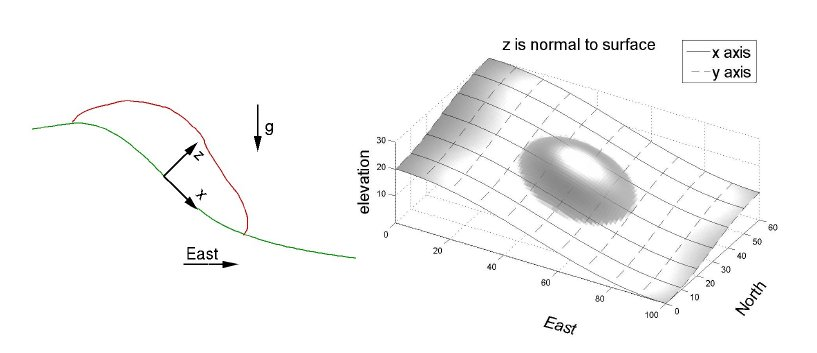
\includegraphics[height=2.8 truein]{IMAGES/1.jpg}
                \caption{In the local coordinate system the {\itshape z} direction is normal to the surface; 
                the {\itshape x} and {\itshape y} directions are tangential to the surface.}
                \label{xzeast}
        \end{center}
\end{figure}
Note that in the momentum equations $k_{ap}g_z\frac{h}{2}h$ is the contribution of hydrostatic 
pressure to the momentum fluxes. $S_h$ is a source of mass, i.e. 
material that either effuses or erodes out of the ground. $S_x$ is 
the sum of a gravitational driving force, the friction that resists motion 
of the material relative to the bed, and the friction that resists the 
internal shearing motion of the material:
\begin{equation}
        \begin{aligned}
                  S_x &=g_x h - \frac{V_x}{\sqrt{V_x^2+V_y^2}}\max\left(g_z+\frac{V_x^2}{r_x},0\right) h \tan(\phi_{bed})
                  - {\rm sgn}\left({\frac{\partial V_x}{\partial y}}\right) h k_{ap} \frac{\partial (g_zh)}{\partial y} \sin(\phi_{int}), \\
                  S_y &=g_y h - \frac{V_y}{\sqrt{V_x^2+V_y^2}}\max\left(g_z+\frac{V_y^2}{r_y},0\right) h \tan(\phi_{bed}) 
                  - {\rm sgn}\left({\frac{\partial V_y}{\partial x}}\right) h k_{ap} \frac{\partial (g_zh)}{\partial x} \sin(\phi_{int}).
         \end{aligned}
         \label{momsourceterms}
\end{equation}
Titan2D solves the above system of equations using a finite volume Godunov method:
\begin{equation}
   \label{integrator}
   U_i^{n+1} = U_i^n - \frac{\bigtriangleup t}{\bigtriangleup x} \{F_{i+\frac{1}{2}}^n - F_{i-\frac{1}{2}}^n \}
   - \frac{\bigtriangleup t}{\bigtriangleup y} \{G_{i+\frac{1}{2}}^n - G_{i-\frac{1}{2}}^n \}.
\end{equation}
In the above equation, G and F are the flux terms at the inter-cell boundaries which are computed by the Harten-Lax-Van Leer (HLL) \cite{Toro2009riemann} Riemann solver that is explained 
in the next section.
\section{SW Solution and Adaptive Strategy for WD Interface }
\subsection{Using Appropriate Riemann Fluxes} \label{Riemann}
Following the recommendation of Toro \cite{ToroBook2001}, TITAN2D uses 
the HLL Riemann average of fluxes. Let $U$ be a state variable, $F$ 
be a flux of that state variable, $s$ be a maximum wave speed, 
and $R$ and $L$ subscripts which denote ``right'' and ``left'' values 
respectively. The HLL Riemann flux is then
\begin{equation}
        F_{HLL}=\begin{cases}
                F_L & s_L\ge 0\\
                F_R & s_R\le 0\\
                \dfrac{s_RF_L-s_LF_R+s_Ls_R(U_R-U_L)}{s_R-s_L} & \textnormal{otherwise}
        \end{cases}
\end{equation}
For the Savage-Hutter system of equations the characteristic speeds are: $s_{1,3}=v\pm a$ and $s_2=v$ where $v$ is the 
velocity of fluid in the corresponding direction and $a=\sqrt{k_{ap}gh}$.
The above HLL solver is not enough for solving this system of equations.
Fraccarollo and Toro \cite{FraccarolloToro1995} note that at the 
wet-dry boundary the Riemann solution consists of a single rarefaction 
wave whose speed (when averaged over the cell length) 
is bounded above by the cell average flow speed plus 
{\bf twice} the ``speed of sound,'' $s=v+2a$, where $a=\sqrt{k_{ap}gh}$ 
for shallow water type granular flows.  They also note that ``an overestimate 
of the true wave speeds results in enhanced stability'' while an 
``underestimate of the true wave speeds could be fatal'' to stability.
They became the first to 
solve this problem by constructing an approximate Riemann solver.
\subsection{Adaptive Meshing} \label{adaptivemeshing}
In TITAN2D each grid cell is a square or very nearly so. Rather than 
using a uniform mesh different sizes of cells are allowed, with each 
successive ``generation'' covering one fourth the area of its ``parent'' 
cell.  Note that only one generation of irregularity is allowed between 
a cell and its neighbors.
At the beginning of the simulation, \textit{i.e.} before the first update, the 
boundaries of all piles are maximally refined. An initial mesh for a 
simulation at Colima Volcano, Mexico, is displayed in Figure \ref{bufcell}. 
\begin{figure}[!h]
        \begin{center}
                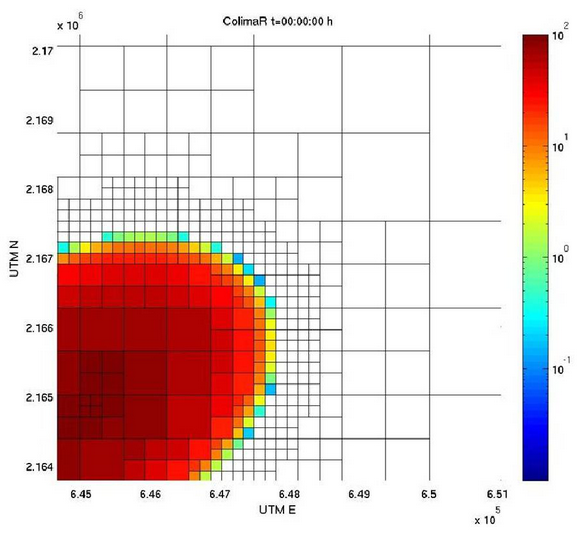
\includegraphics[scale=.3]{IMAGES/buffercells.png}
                \caption{Buffer cells. \red{A BETTER CAPTION IS NEEDED.}}
                \label{bufcell}
        \end{center}
\end{figure} 
During normal adaptivity cells are selected for refinement if they meet 
either of two requirements:
\begin{enumerate} 
        \item They have large, as compared to the average, inter-cellular fluxes. \footnote{More systematic error estimate driven approaches have been tried \red{THIS NEEDS A CITATION}\cite{} but 
        empirical experience suggests that these simple indicators provide sufficient information for reliable and fast simulations.}
        \item They are at or within a few cells near the interface.
\end{enumerate}
The former condition allows for the accurate capture of sharp changes in state variables. The latter results in banded regions of the flow separated into ``rings'' of maximally refined buffer cells.  
This limits artificially high transportation of material from the inside of the interface to outside of the interface and guarantees that material will only flow into maximally refined dry 
cells at the wet-dry front.
However, some material that are outside of the recognized boundary may be left outside the outermost band of buffer cells. These cells are not updated until the interface passes them.
The rings of buffer cells strategy decreases the numerical wicking problem and when combined with interface capturing scheme it is sufficient to decrease other thin layer problems to a level that 
prevents the loss of stability.
Clearly this strategy depends on the way that we describe the interface. In the heuristic approach, after using a threshold to find the wet and dry areas the number of rings are a number of cells wide 
equal to or greater than the number of iterations between mesh adaptations (we adapt the mesh after every 5 to 10 time steps). In the level set approach we can use a narrow band method for adaption 
and selecting of these buffer rings, but we simply select the elements such that their distance to the interface are less than a normalized distance that is obtained from the maximum distance 
to the interface. Note that in the level set method distance of the cells to the interface is the level set function itself and we do not pay any additional computational cost for that information. 
In the phase field method we have a diffusive region between two phases that we can control with a capillary width (please refer to section \ref{phase field}).
We are thus able to select those cells such that $|\phi| <1 $ where $\phi$ the phase field value. We set the capillary width equal to the number of time steps between successive adaptivity steps.
Unrefinement takes place immediately after refinement; a group of four ``sibling'' cells will be selected to merge into their mutual ``parent'' cell if the sum of their inter-cellular fluxes is very 
low compared to the average flux.  Cells that have either just been refined or are otherwise in any of the current bands of buffer cells are immune 
to unrefinement.  
    
\section{Interface Capturing Strategies}\label{solution}
In the aforementioned parts the major difficulties of numerical analysis of the shallow water
equations were discussed, and it was shown that most of them are directly or indirectly related to the WD problem.
For more intuition, the result of a simulation for Atenquique debris is displayed in figure \ref{thinlayerproblem}. 
The left picture is the obtained result from the solver and the right picture is the same result, but flow height is displayed 
only for flow height greater than 0.5 $m$. This picture shows for the pure solver the dominant part of the 
domain is filled with negligible flow depth and this makes the actual interface mix with the thin layer region.
In this section three methods to solve the WD problem which mitigate the numerical difficulties of SWE are explained. 
\subsection{First: Heuristic methods} \label{Heuristic}
Usually, heuristic methods use one or a combination of the following four strategies \cite{Medeiros2013}: 
\begin{enumerate}
        \item Filling the entire computational domain with a thin layer of fluid,
        \item Using a depth scale to check whether a cell or a node is wet or dry 
         (or possibly partially wet), and then  making a decision to add or remove it 
         from the computational domain,
        \item Employing some extrapolating scheme from the wet cells into their neighbor 
         cells to approximate the location of the interface. This method is usually called 
         volume/free-surface relationship (VFR) in the literature,
        \item Permitting fluid height to be negative, which means that it is below the topographical surface.
\end{enumerate}
Table \ref{table1} compares these heuristim methods.
\begin{center}\label{table1}
        \begin{tabular}{|c|p{5cm}|p{5cm}|}
                \hline
                {\bf Strategy}                  & {\bf Mass Conservation}                                          & {\bf Physics} \\
                \hline
                {\bf Thin film}                 & Adequate, but requires solution reconstruction 
                & Produces a smooth and realistic wetting front     \\
                \hline 
                {\bf Cell removal}              & Dependent on numerical method for solving the equations          & Excellent, performs better on advancing front than receding front \\
                \hline
                {\bf VFR}                       & Conservative, with aid of some correction procedure              & Very good in wide verity of problems      \\
                \hline
                {\bf Allowable negative depth}  & Conservative, but performance depend on WD parameters            & Same as mass conservation      \\
                \hline
                % \caption{Comparison of different strategies for WD problem in SWE}
        \end{tabular}
\end{center}
\red{What is the heuristic method that is actually used? This is not stated yet.}
\subsubsection{Selecting appropriate threshold} \label{Threshold}
In this approach we use a very small threshold for flow height to segregate the wet, partially wet and dry cells.
The critical contribution of this scaling is to allow other
facets like flux adjustment and boundary reconstruction to identify where the flow %is merely ``thin'' and where it 
is non-physically thin, \textit{i.e.} where should they consider the boundary of
the flow to be. Consistency is the key requirement of whatever strategy we choose to
determine the scaling. That is, the
chosen strategy must be able to generate the same ``appropriate'' value
for depth scale at the beginning and at the end of a simulation.  
In a ``typical'' geological simulation, say of the collapse of a volcanic 
dome which would be modeled in TITAN2D as a``pile source'', the initial 
body of mass can be quite deep, but at the end of the simulation the 
material will likely be spread over a large area.  Hypothetically, if one 
were to scale by maximum flow depth at the beginning and end of the 
simulation, they would obtain vastly different values.  More importantly, 
if the only source of mass was an effusion of material out of the ground, 
the maximum initial flow depth would be zero, even if the total volume 
during the course of the simulation was the same as the previously 
mentioned ``pile source''.  
On the other hand, scaling by the cube root of the total volume of the 
flow being simulated is entirely consistent and is the flow depth 
scaling factor used by TITAN2D.  We do {\bf not} claim that the cube root 
of volume is any more or less appropriate as a scaling factor than 
maximum initial flow depth in other shallow water contexts, for example 
storm surge simulation.
Having chosen a consistent scaling factor we were then able to define 
associated non-dimensional depths for negligibly thin and merely thin
flows.  If one were to assume that a particular geophysical mass flow 
event involved a volume of $10^8 [{\rm m}^3]$, it would then be 
reasonable to state that flow depths of less than $5 [{\rm cm}]$ were
both negligible and non-threatening.  This roughly equates to 
non-dimensional negligible flow depth, which we call 
{\rm\verb1GEOFLOW_TINY1}, with the value 
\begin{equation}
{\rm\verb1GEOFLOW_TINY1} = 0.0001.
\end{equation}
Using this value, and assuming
the volume used in a laboratory scale test was $1 [{\rm cm}^3]$, the 
resultant negligible flow depth would be $0.0001 [{\rm cm}]$.  As can 
be observed from these two examples, the chosen value of 
{\rm\verb1GEOFLOW_TINY1} is physically appropriate across a very large 
range of volumes.  We therefore use a theoretical contour at this depth 
as the boundary of the simulated flow.  %
%     \subsubsection{Thresholding} \label{thresholding}
In the introduction section we stated that unless steps are taken to 
prevent it, the numerical wicking (Problem \ref{problemwicking}) will
cause the flow to spread 1 cell every time-step even though the product
of flow speed and time-step size is less than the cell length.  In 
addition, the familiar continuum equations loose hyperbolicity (wave 
speeds tend to infinity) at the boundary between a continuous material 
and a vacuum.  Having implicitly defined the flow boundary,
we prevent calculation of state variables outside the flow, \textit{i.e.} in 
regions with flow depth below {\rm\verb1GEOFLOW_TINY1}.  
This reduces both non-physical flow 
spreading and computational cost. Note that state variables in cells 
with flow depth less than {\rm\verb1GEOFLOW_TINY1} are {\bf not} zeroed.  
% Once having made the the decision to implement the negligible flow 
% depth threshold, one is faced with choosing a value for the threshold.
% If the chosen threshold is overly large, it would impose a non-physical 
% limit to the flow.  Consequently, the previously stated value of 
% {\rm\verb1GEOFLOW_TINY1} was chosen with the intention of being 
% conservatively low.  However, this results in the negligible flow 
% depth threshold not being able to entirely circumvent the loss of 
% hyperbolicity (Problem \ref{problemunstableB} from Subsection 
% \ref{CausesSubSec}).  We compensate for this through appropriate Riemann 
% fluxes. Thresholding also decreases the numerical wicking (Problem 
% \ref{problemwicking}) at the flow boundary.
\subsubsection{Interface Reconstruction} \label{Interfacerecon}
As noted above, the use of a standard Eulerian grid imposes discrete 
fixed increments to the flow extent which contributes to the wicking problem
(Problem \ref{problemwicking} ) at the 
boundary.  Use of adaptive mesh refinement 
reduces this error by reducing the amont of the increment. 
The Lagrangian approach does not have this 
limitation, which Tai et al. \cite{Tai2002} took advantage
of when they augmented their one dimensional NOC scheme with 
Lagrangian front tracking.  However, implementing a hybrid 
Eulerian-Lagrangian scheme in two dimensions is significantly more 
complex. 
Therefore, as part of our multi-faceted approach we implemented a very 
simple and inexpensive interface reconstruction and predictive 
Lagrangian front tracking scheme.  Knowledge of the interface allows
us to generate a representative average for an individual cell edge 
over the time-step and for values of state variables which are then used to 
compute inter-cellular fluxes into/out-of partially wet cells.  The 
interface reconstruction scheme is illustrated in figure \ref{interface}.
\begin{figure}[!h]
        \centerline{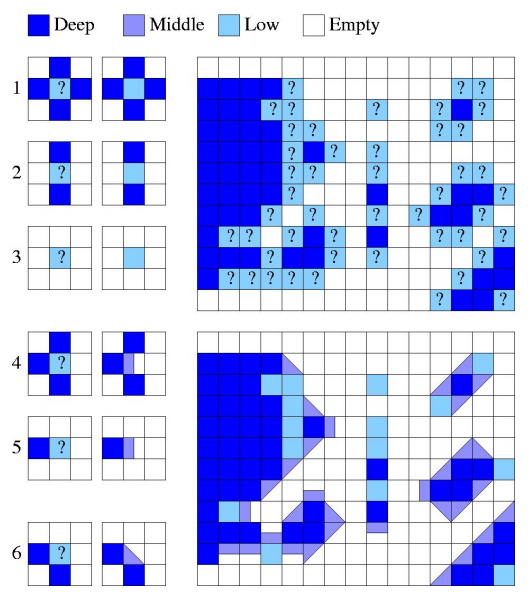
\includegraphics[scale=0.3]{IMAGES/flux.png}}
        \caption{Interface Reconstruction in TITAN2D}
        \label{interface}
\end{figure} 
%\clearpage
Specifically, each partially wet cell is assumed to be split by a 
straight line into a completely dry and a completely wet part.  For the 
sake of simplicity, we restrict this line to one of four orientations: 
east-west, north-south, or parallel to either diagonal of the square
cell.  However, all placements/translations of the wet-dry line are 
allowed.  At the beginning of each time-step, the orientation of the 
line for the entire time-step is set based solely on which of the cell's 
neighbors have flow depth greater/less than the {\rm \verb1GEOFLOW_TINY1} 
threshold\footnote{As stated in Subsection \ref{adaptivemeshing}, the 
refinement strategy ensures that the flow front will always be maximally 
refined.  This simplifies the coding since all cells at the front can be
safely assumed to have only one neighbor on each side.}.   Orientation
of the wet-dry line, and which side of it is wet, is indicated by a single 
integer representing the geometrically determined ``most wet node.'' 
The only nine possible values for the most wet node are any of the 
cell's corners, edge midpoints or its center.  The most wet node is 
assumed to have a flow depth that is the maximum of the cell or any of 
its four neighbors.  The placement of the line is such that the volume of 
material in the cell under a plane passing through the most wet node
and the wet dry-line is the same as the unadjusted cell.  %Knowing the 
%wet-dry line's placement, the wet part only average of a conservative 
%state variables equals its whole cell average value divided by the 
%fraction of the cell's area that is wet.
Since we now know where the wet-dry line is at the beginning of the 
time step, we can compute which of the cell's edges are completely 
wet, completely dry, or partially wet, and the fraction of wetness for 
the partially wet edges.  Given the orientation and beginning of 
time-step location of the wet-dry line and the cell's state variables, 
it is also fairly straight forward to predict the line's end of 
time-step location.  This is done by convecting the wet-dry line at 
the shock speed, $s=v+a$ where the speed of sound has been adjusted 
to account for only part of the cell being wet, i.e. 
$a=\sqrt{k_{ap}gh\frac{A}{A_{wet}}}$.  Here $A$ is the whole cell's 
area and $A_{wet}$ is the portion of the cell's area that is wet.  
Since the wet-dry boundary within each partially wet cell is assumed 
to be a straight line with, during the time-step, fixed orientation, 
convecting a single point, in this case the midpoint, on the line is 
equivalent to convecting the entire wet-dry line.  A spatial and time 
average of the wetness factor for the edge over the time-step can 
therefore be easily computed as
\begin{equation}
        W=\left(\frac{0\cdot\Delta t_{dry} +\frac{1}{2}(w_{beg}+w_{end})\Delta t_{part}+1\cdot\Delta t_{wet}}{\Delta t}\right) \left(\frac{A}{A_{wet}}\right)
        \label{wetnessfactor}
\end{equation}
where $\Delta t=\Delta t_{dry}+\Delta t_{part}+\Delta t_{wet}$ is the 
entire time-step, $\Delta t_{dry}$ is the portion of the time-step for 
which the edge is completely dry, $\Delta t_{part}$ is the portion of 
the time-step for which the edge is partially wet and partially dry, 
$\Delta t_{wet}$ is the portion of the time-step for which the edge is 
completely wet, $w_{beg}$ is the edge's fraction of wetness at the 
beginning of the time-step, and $w_{end}$ is the edge's fraction of 
wetness at the end of the time-step.
\subsubsection{Adjusting Fluxes in Partially Wet Cells} \label{adjustfluxes}
The state variables used to compute the physical fluxes are the whole
cell average values multiplied by the edge wetness factor.  Note this 
results in the zeroing of this cell's physical fluxes for its sides 
that will be completely dry for the entire time-step and increasing 
them for sides that will be completely wet for the entire time-step.   
The numerical fluxes are then taken to be the HLL Riemann average of 
the ``adjusted'' physical fluxes from the cells on both sides the edge.  
The wetness factor adjustment of fluxes delays/decreases the transfer 
of material from partially wet cells to completely dry cells.  This 
delay significantly reduces the amount of non-physical flow spreading, 
and requires negligible additional computation and memory usage.  In 
terms of memory usage, this scheme only requires one additional
integer indicating the most wet node, and two additional decimal 
numbers for the cell's fraction of wet area and the location of the 
wet-dry line's midpoint (implemented as a single number ranging from 
zero to one).  The flux adjustment in partially wet cells mitigates
the numerical wicking (Problem \ref{problemwicking}) at the boundary but not within the flow (that
requires either a uniform grid or an adaptive strategy based on
fluxes and the rings of buffer cells strategy).
% 
% {\bf 1D Analysis of partially wet flux adjustment}
% 
% There are 3 cells L, M, R.  $h_R=V_R=0$, $h_L>2 h_M>0$ (the middle cell is partially wet), $V_L>0$, $V_M>0$.  The timestep is set by the middle cell with a Courant number $C$. 
% 
% The wet area of the {\it partially wet} middle cell is defined as follows
% \begin{eqnarray}
% h_m A &=& \frac{1}{2} h_L A_wet  \\
% \frac{A_{wet}}{A} &=& 2\frac{h_m}{h_L}
% \end{eqnarray}
% More generally 
% \begin{equation}
% \frac{A_{wet}}{A}=\min\left(1,2\frac{h_m}{h_L}\right)
% \end{equation}
% We can then compute a wet portion average of $h$ and $hV$ for the middle cell
% \begin{eqnarray}
% \hat{h}_m&=&h_m\frac{A}{A_{wet}} \\
% \widehat{(hV)}_m &=& hV\frac{A}{A_{wet}}
% \end{eqnarray}
% The adjusted wave speeds in the middle cell are $s=V_m \pm 2\alpha\sqrt{\hat{h}_m}=V_m \pm 2 \alpha \sqrt{h_m} \sqrt{\frac{A}{A_{wet}}}$.  This makes the timestep
% \begin{equation}
% \Delta t = C \frac{\Delta X_m}{V_m+2\alpha\sqrt{h}\sqrt{\frac{A}{A_{wet}}}}
% \end{equation}
% The wet-dry line can then be convected at $s=V_m+2\alpha\sqrt{h_m}\sqrt{\frac{A}{A_{wet}}}$ and the time at which the flow will reach the edge of middle and right cells.   
% \begin{eqnarray}
% \Delta t_{part} &=& \min\left(\Delta t, \frac{\Delta X_m \left(1-\frac{A_{wet}}{A}\right)} {V_m+2\alpha\sqrt{h}\sqrt{\frac{A}{A_{wet}}}}\right) \\
% \Delta t_{wet}&=&\Delta t - \Delta t_{part} 
% \end{eqnarray}
% We can then define a time averaged wetness factor, $W_{MR}$ for the middle cell for the edge shared by the middle and right cells
% \begin{eqnarray}
% W_{MR}&=&\frac{\Delta t_{wet}}{\Delta t} \frac{A}{A_{wet}}\\
% &=&\left(1-\frac{\Delta t_{part}}{\Delta t}\right)\frac{A}{A_{wet}}\\
% &=&\frac{A}{A_{wet}}-\min\left(\frac{A}{A_{wet}},\frac{\frac{\Delta X_m}{\Delta t} \left(\frac{A}{A_{wet}}-1\right)}{V_m+2\alpha\sqrt{h}\sqrt{\frac{A}{A_{wet}}}}\right)\\
% W_{MR}&=&\frac{A}{A_{wet}}-\min\left(\frac{A}{A_{wet}},\frac{1}{C}\left(\frac{A}{A_{wet}}-1\right)\right)
% \end{eqnarray}
% Then 
% \begin{eqnarray}
% F_{hMR}^*&=&\frac{\left(V_m+2\alpha\sqrt{h_m}\sqrt{\frac{A}{A_{wet}}}\right)W_{MR}h_mV_m-\left(V_m^2-4\alpha h_m\frac{A}{A_{wet}}\right)W_{MR}h_m}{4\alpha\sqrt{h_m}\sqrt{\frac{A}{A_{wet}}}}\\
% &=&\frac{W_{MR}h_m}{2}\left(V_m+2\alpha\sqrt{h}\sqrt{\frac{A}{A_{wet}}}\right)
% \end{eqnarray}
% Likewise 
% \begin{eqnarray}
% F_{hVMR}^*&=&\frac{\left(V_m+2\alpha\sqrt{h_m}\sqrt{\frac{A}{A_{wet}}}\right)\left(W_{MR}h_mV_m^2+\frac{1}{2}\alpha^2W_{MR}^2h_m^2\right)-\left(V_m^2-4\alpha h_m\frac{A}{A_{wet}}\right)W_{MR}h_mV_m}{4\alpha\sqrt{h_m}\sqrt{\frac{A}{A_{wet}}}}\\
% &=&...
% \end{eqnarray}
% 
% The middle cell's wetness factor, $W_{ML}$, for the edge shared with the left cell is
% \begin{equation}
% W_{ML}=\frac{A}{A_{wet}}
% \end{equation}
% Note that if the wet-dry line does not reach the edge shared by the middle and right cells within the timestep then $W_{MR}=0$.  Assuming that this is the case then
% $h_R'=V_R'=0$ and ... 
% $h_M'$, and $V_M'$ also depend on $h_L$ and $V_L$ so their values must be known/assumed in order to compute/simplify $h_M'$ and $V_M'$
\subsection{Second: Phase Field Method} \label{phase field}
As noted earlier, another approach that is employed 
for capturing the interface of a SW type flow is the phase field method.
In this method the state variables are augmented by a continuous
order parameter. This order parameter, $\varphi$, 
implicitly represents the interface in the domain. To this aim, a new transfer equation must be solved which is coupled with the other state variables. 
Papers \cite{Chen2002,Anderson1998,Boettinger2002,Kim2012} are good references about the history and evolution of the method.
Phase diffusion methods and particularly the phase field method is based upon the notion that the interface between phases is a diffusive region rather than a sharp interface. 
The value of $\phi$ is constant within a bulk phase but changes smoothly between the phases. In this work $\phi$ is 1 for the fluid phase $ \lbrace \textbf{x}: \phi(\textbf{x},t)=1 \rbrace  $, 
and it is -1 for void regions $ \lbrace \textbf{x}: \phi(\textbf{x},t)=-1 \rbrace  $, and is between -1 to 1 on the diffusion region $ \lbrace \textbf{x}: -1 < \phi(\textbf{x},t) < 1 \rbrace  $. 
We can implicitly assume the interface of the flow is where $ \lbrace \textbf{x}: \phi(\textbf{x},t)= 0 \rbrace  $.
%The strong thermodynamical and physical derivation of the method make it so powerful for capturing the complicated topological changes especially for the problems that the interface motion depends 
%on gradients of an external field normal to the interface and on the local curvature of the interface.
In this study we used Allen-Cahn form of the phase field. 
\begin{equation} 
        \label{allencahn}
        \frac{\partial \varphi }{\partial t} + \overrightarrow{V}\cdot \nabla \varphi = 
        \gamma (\bigtriangleup\varphi -F'(\varphi)),
\end{equation}
where
\begin{equation} 
        \label{fprime}
        F(\varphi)=\frac{1}{4\eta^2} (\varphi^2-1)^2 ,\text{\ so \ \ } F'(\varphi)= \frac{\delta F}{\delta \varphi} = \frac{1}{\eta^2} \varphi (\varphi^2 -1).
\end{equation}
In above equation $\eta$ is a constant that regulates the capillary width or diffusion width, and $ \gamma $ denotes an elastic relaxation constant, and $F(\varphi)$ is 
a mixing free energy which is the well-known double-well potential function, and represents the interactions of different volume fractions of individual species \cite{Bronsard1990,Larson1999}.
This formulation is easier to solve, but is not mass conservative, to conserve the mass a Lagrange multiplier in form of $(\varphi^2-1)\xi(t)$ is added as a source term to the right hand side of equation \eqref{allencahn}. The reason that we select this form for the Lagrange multiplier is because we do not want to change $\varphi$ on the bulk region as well as when on the interface i.e when $\varphi=\pm1$. So the final for of equation $\xi(t)$ would be:  
\begin{equation} 
        \label{allencahn_mod}
        \frac{\partial \varphi }{\partial t} + \overrightarrow{V}\cdot \nabla \varphi = 
        \gamma (\bigtriangleup\varphi -F'(\varphi)+ (\varphi^2-1)\xi(t)),
\end{equation}
and the constrain that has to be satisfied is:
\begin{equation} 
        \label{constrain}
        \frac{D}{Dt} \int_\Omega \varphi h \ \ dx= 0,
\end{equation}
which basically means the initial volume of pile must be constant during the simulation. Consequently $\xi(t)$ is derived as follow:
\begin{equation} 
        \label{eta}
        \frac{D}{Dt} \int_\Omega \varphi h \ \ dx= h \int_\Omega \frac{D}{Dt}  \varphi  \ \ dx+\underbrace{\varphi \int_\Omega  \frac{D}{Dt} h  \ \ dx}_{=0 \text{\ \ continuity}}=h\int_\Omega \gamma (\bigtriangleup\varphi -F'(\varphi)+\varphi (\varphi^2-1)\ \xi(t)) \ \ dx,
\end{equation}
the first term in above relation will be neglected by applying the Gauss' theorem with considering the boundary conditions($
        \frac{\partial \varphi}{\partial n}\vert_{\Gamma} = 0,
$):
\begin{equation}
        \label{lapbound}
        \int_\Omega h \gamma  \nabla. \nabla \varphi \ dx = 
        \int_\Gamma h \gamma \nabla \varphi \ ds = 0,
\end{equation}
so to always satisfy the constrain \eqref{constrain} we end up with:
\begin{equation} 
        \label{eta_cont}
\frac{1}{\eta^2} \int_\Omega  \varphi (\varphi^2 -1) \ \ dx = \xi(t) \int_\Omega (\varphi^2-1)  \ \ dx \Rightarrow \xi(t) = \frac{\int_\Omega  \varphi (\varphi^2 -1) \ \ dx}{\eta^2 \int_\Omega (\varphi^2-1)  \ \ dx }
\end{equation}
We set $\eta=n\  \delta x$, where $\delta x$ is equal to the smallest cell length of all elements and $n$ is the number of the buffer layers explained in section \ref{adaptivemeshing}.
Form time integration of equation \eqref{allencahn_mod} we use operator splitting to get benefit of propper scheme for each part of the equation. We use the Euler explicit method for time integrarion of all terms except the laplacian terms, and update the Laplacian term by the Euler implicit scheme. The length of time step is based on CFL condition for the explicit scheme. 
\begin{align}
\frac{\varphi^{i+.5}-\varphi^i}{\bigtriangleup t}&= \gamma (-F'(\varphi^i)+\varphi^i (1-(\varphi^i)^2)\ \xi(t^i)) \label{eq1.exp}\\
\frac{\varphi^{i+1}-\varphi^{i+.5}}{\bigtriangleup t} &= \gamma \nabla .\nabla \varphi^{i+1} \label{eq2.exp}
\end{align}
We used GMRES solver of the PETSc \cite{petsc-user-ref} library to solve equation \eqref{eq2.exp}. Since the Krylov subspace solvers just needs the result of matrix-vector multiplication, we used matrix-free method to compute the laplacian term to decrease the memory cost of implicit solver.
\subsection{Third: Level Set Method} \label{level set}
The last method that we use to capture the interface for a SW flow is the Level set method.
The Level set method is another Eulerian interface capturig method; it was introduced by Osher and Sethian in 1988 \cite{Osher1988}.
The basis of the method is to capture the interface by means of solving a hyperbolic Hamilton-Jacobi PDE on 
the computational domain which follows the boundaries. The level set variable $\varPsi (X,t)$ implicitly represents the interface. In this method, $\varPsi (X,t)$ is a signed distance function which means it is zero on the interface, and its absolute value changes in the domain with respect to the distance to the zero level, and its sign is positive outside of the interface, and is negative inside of the interface. 
Given the initial condition $\varPsi (X,t)_0$ the advection of the interface ($\varPsi (X,t)=0$) only depends on the normal velocity $F$:
\begin{equation}\label{levelseteq1}
        \frac{\partial \varPsi}{\partial t} + F |\nabla \varPsi| = 0,
\end{equation}
substituting $F = \overrightarrow{V} \overrightarrow{n} $ which  $\overrightarrow{n} $ is the normal vector, and is equal to
$ \frac{\nabla \varPsi}{|\nabla \varPsi|}$ leads to:
\begin{equation}\label{levelseteq2}
        \frac{\partial \varPsi}{\partial t} + \overrightarrow{V} \nabla \varPsi = 0
\end{equation}
\subsubsection{Reinitialization} \label{reinitialization}
Solution of equation \eqref{levelseteq2} is not essentially a signed distance function, to keep $\varPsi$ a signed distance function, we need a procedure that is called initialization or reinitialization. There are several techniques for this purpose \cite{Osher1988}, but what we implemented here is a composition of the method presented in Chopp's work \cite{Chopp2001} with some modifications, for the points close to the interface, and a PDE based initialization for the further places\cite{Sussman1994a}.

PDE based initialization is easy for parallelization, though it suffers from preserving the interface location that causes loose of conservation mass/area. Chopp's suggests a bicubic interpolation for the points near the interface \cite{Chopp2001}, but here we use a bilinear interpolation which is not as accurate as what he suggested, but it is accurate enough to preserve the interface. For further distances we do not need very accurate $\varPsi$, so we use a PDE based reinitialization which is easier to implement and has lower computational cost. In our approach, we first find $\varPsi$ for the points that are adjacent to the interface, then use these points to update the signed distance function for rest of the points by PDE based initialization. In this way, the interface $( \varPsi=0 )$ is preserved with an afordable computational cost and effort. Moreover, since just $\varPsi$ is required for the points that are located near the interface, there is no need to update it for whole of the domain, so in this work we select $\varPsi_{thresh}<10\ \delta x$, which  $\delta x$ is the smallest size of the elements, as the threshold for updating $\varPsi$ in the initialization.

The signed distance function is updated for adjacent points to the interface in following steps:
\begin{enumerate}
\item First we find the adjacent points to the interface, and store them in a list that is usually called accepted points list in the literature \cite{Chopp2001}. 
\item Second step is to find an interpolation for a level set function $p(X)$ that returns $\varPsi(X)$ given the position of the points. 
\item The last step is to compute the distance of accepted points based on the following conditions:
\begin{subequations}
\begin{align}
&p(X_{int})=0,\label{dist_cond1} \\ 
&\nabla p(y) \times (X_0-X_{int})=0,\label{dist_cond2}
\end{align}
\end{subequations}
where $X_{int}$ is the nearest point on the interface, and $X_0$ is the point in the accepted list that we want to compute its distance to the interface. First condition \eqref{dist_cond1} basically means that $X_{int}$ is on the interface, and the second condition says that if we draw a line from $X_0$ to closest point on the interface, it has to be perpendicular on intersection point with the interface. In this part, we followed the notation of Chopp's paper \citep{Chopp2001}.
\end{enumerate}

In the first step, we just need to find those points that sign of $\varPsi$ is different from their neighbors, and store them in a list that we call them accpeted points list. 

For the second step, there are different ways for interpolation through the accepted points and finding $p$. In many applications, like in this study, initial interface has a specific geometrical shape like circle or ellipse, so we do not need to find it approximately, and its equation can be used directly as $p(X)$. For example, in this study initial pile has elliptic shape, so the initial interface follows elliptic equation. If we do not know the equation of the interface which is usually the case, especially in the reinitialization, we need to find $p$ by interpolation. Chopp's suggested a bicubic approximation \cite{Chopp2001} to achieve a fully second order accurate  result, but his method yields to solve a 16 by 16 system of equations for every four neighbor points in the accepted list to find the coefficient of the bicubic interpolation. Since the whole point of this interpolation is to compute the distance to the interface more accurately, in order to preserve the location of the interface, in this study instead of bicubic approximation we used a bilinear interpolation. So the general form of $p$ is:
\begin{equation}\label{interpolation}
p=a_0+a_1 \ x+ a_2 \ y+ a_3 \ xy.
\end{equation} 

To find $a_0$ to $a_3$ we just need to solve a system of 4 by 4 equations resulted from value of $\varPsi$ and the position of the points. After finding $p$, we can compute the distance from equation \eqref{dist_cond1} and \eqref{dist_cond2}. These equations form a nonlinear system of equations that we use a variant of Newton's method presented in \cite{Chopp2001} to solve them:
\begin{subequations}
\label{eqnewton}
\begin{align}
&\delta_1=-p(X^k)\frac{\nabla p(X^k)}{\nabla p(X^k).\nabla p(X^k)},\\
& X_{1+\frac{1}{2}}=X_k+\delta_1,\\
& \delta_2=(X^0-X^k)-\frac{(X^0-X^k).\nabla p(X^k)}{\nabla p(X^k).\nabla p(X^k)}\nabla p(X^k),\\
&X_{k+1}=X_{1+\frac{1}{2}}+\delta_2,
\end{align}
\end{subequations}
equation \eqref{eqnewton} is an iterative method that starts from $X_0$ which is the point that we want to find its distance to the interface. Clearly, above equation gives the nearest point on the interface, and then the distance can be computed, and sign of $\varPsi$ is same as what it was before reinitialization.
For interpolation in \eqref{interpolation}, we need four points. When we create accepted list, instead of storing points we store a pair of points that are neighbor and their sign of $\varPsi$ is different. Then to find two other points, it is enough to select a direction and find the neighbors of the first two points in the selected direction. Since we use AMR with structured grid in TITAN2D, the selected four points creates a quadrilateral (and not essentially a rectangle or squre) that are used for the interpolation.

Our experience shows using set container of C++ standard library is a very proper data structure for storing the adjacent points near the interface in the first step. The reason is that this container keeps its item in a sorted way, and does not let to store duplicated items. So when we search to find those neighbors that have different $\varPsi$ signs to store them in the list, we will not worry to store an element more than once, and there is no need to check the list everytime that we want to save a new element to make sure that we have not saved it before. Only thing that one has to do is to overload the less operator by the desired properties of the elements, that could be element's position or key, to have a sorted list with the unique items.

After finding $\varPsi$ for the points adjacent to the interface, $\varPsi$ in other points can be updated with a PDE based reinitialization in an unwinding scheme. We used the following PDE for this aim:
\begin{equation}\label{initializationeq}
        \frac{\partial \varPsi}{\partial \tau} + \sgn (\varPsi_0) (|\nabla \varPsi| - 1)= 0 
\end{equation}
In equation \eqref{initializationeq} $\tau$ is a pseudo-time and the equation should be solved until it converges reasonably. This PDE adjusts $\varPsi$ such that $|\nabla \varPsi|=1$.
We solve equation \eqref{initializationeq} by the method introduced in \cite{Adalsteinsson1999}. 
\begin{equation}
        \varPsi_{ijk}^{n+1}=\varPsi_{ijk}^{n}-\bigtriangleup t \left(max(F,0)\bigtriangledown_{ijk}^{+}+min(F,0)\bigtriangledown_{ijk}^{-} \right),
\end{equation}
where 
\begin{equation}
        \begin{aligned}
                \bigtriangledown_{ijk}^{+} = \big[ & \max(D^{-x}\varPsi_{ijk}^{n})^2 + \min(D^{+x}\varPsi_{ijk}^{n})^2
                \\& \max(D^{-y}\varPsi_{ijk}^{n})^2 + \min(D^{+y}\varPsi_{ijk}^{n})^2 \big]^{1/2}
        \end{aligned}
\end{equation}
 
\begin{equation}
        \begin{aligned}
                \bigtriangledown_{ijk}^{-} = \big[ & \min(D^{-x}\varPsi_{ijk}^{n})^2 + \max(D^{+x}\varPsi_{ijk}^{n})^2
                \\& \min(D^{-y}\varPsi_{ijk}^{n})^2 + \max(D^{+y}\varPsi_{ijk}^{n})^2 \big]^{1/2}
        \end{aligned}
\end{equation} 
In the above equations $D^+$, and $D^-$ are  respectively the backward and forward differences in the corresponding directions.
We solve equation \eqref{initializationeq} until we reach the convergence or make sure that we have updated the points far enough from the interface. The threshold that we used for convergence was $.5 (\delta x)^3$.
\section{Results} \label{results}
\subsection{Inclined plane}
In this section the results of the study is presented in the same order they were introduced in the paper.
Table 1 shows the applied initial condition for these results.
\begin{center}
        \begin{tabular}{|l|c|}
                % \caption{Initial condition}
                \hline
                Maximum pile height       & .061 m \\
                \hline
                Major extent of the pile  & .0525 m \\
                \hline
                Minor extent of the pile  & .0525 m \\
                \hline           
                Bed friction angle        & $32.47^o$ \\
                \hline
                Internal friction angle  & $37.3^o$ \\
                \hline
                Angle of incline          & $38.5^o$ \\
                \hline
        \end{tabular}
\end{center}
\begin{figure}[H]
        \begin{minipage}[b]{.48\linewidth}
                \centering
                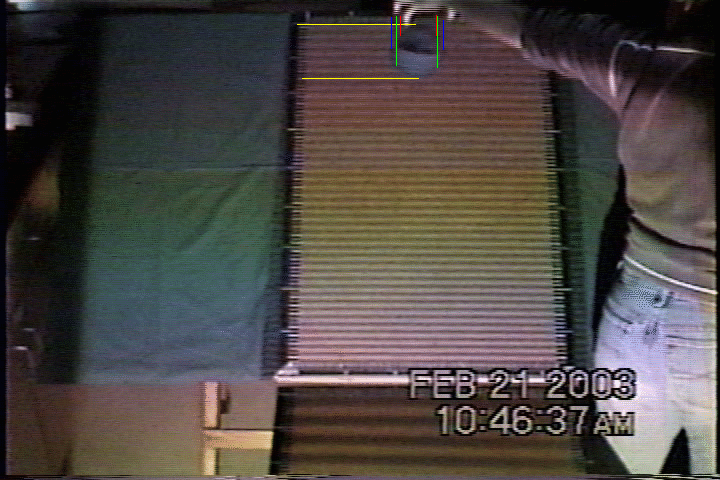
\includegraphics[width=1\textwidth]{IMAGES/expinitialconf.png}
                \subcaption{Experimental setup}
        \end{minipage}
        %   \hfill
        \begin{minipage}[b]{.48 \linewidth}
                \centering
                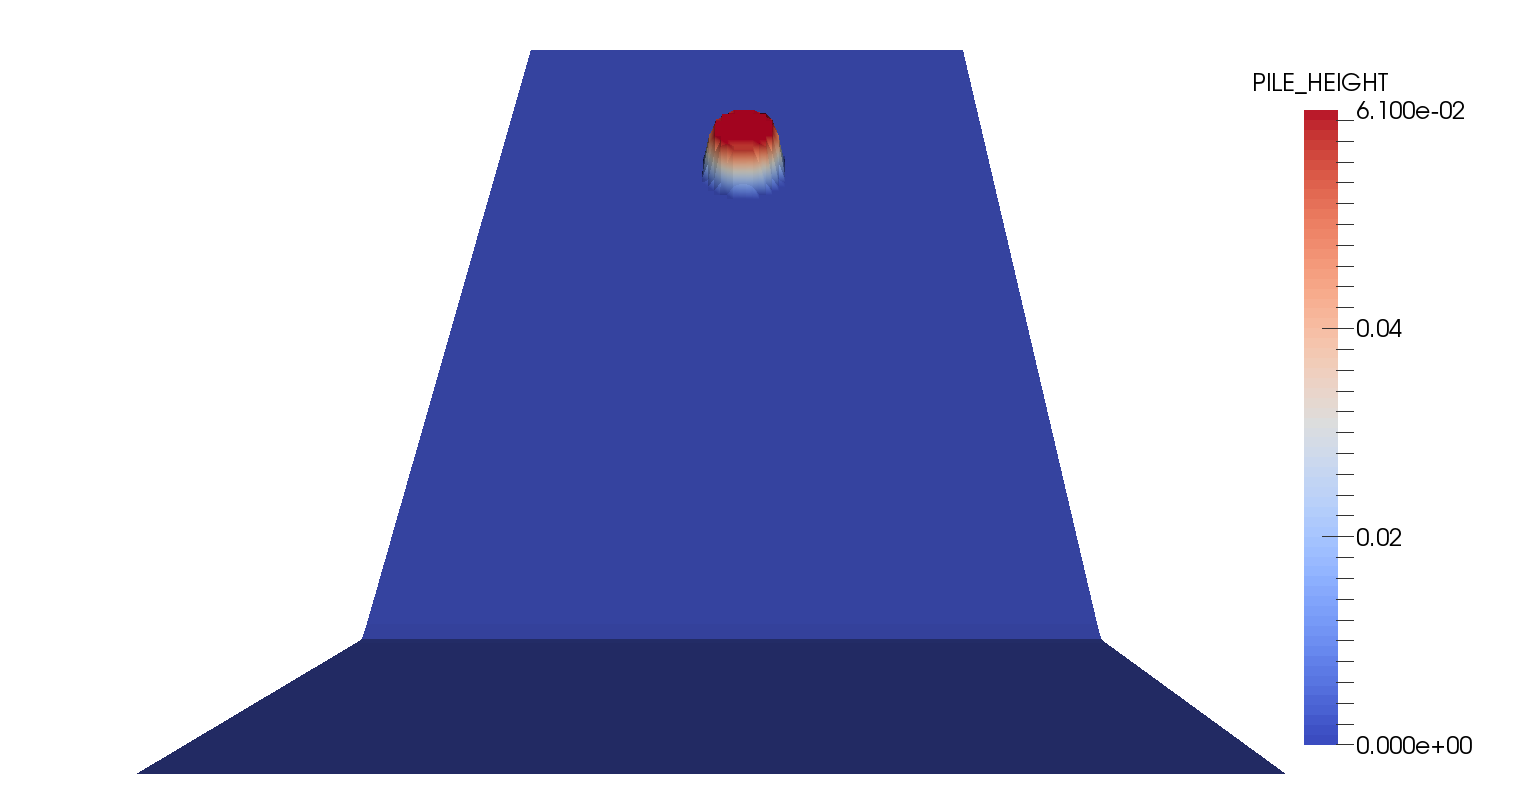
\includegraphics[width=1\textwidth]{IMAGES/initialconf.png}
                \subcaption{Numerical simulation}
        \end{minipage}
        \caption{Initial configuration of the pile on the incline}
        \label{initialconf}
\end{figure}
%\subsubsection{Heuristic Method}
\begin{figure}[H]
        \begin{minipage}[b]{.48\linewidth}
                \centering
                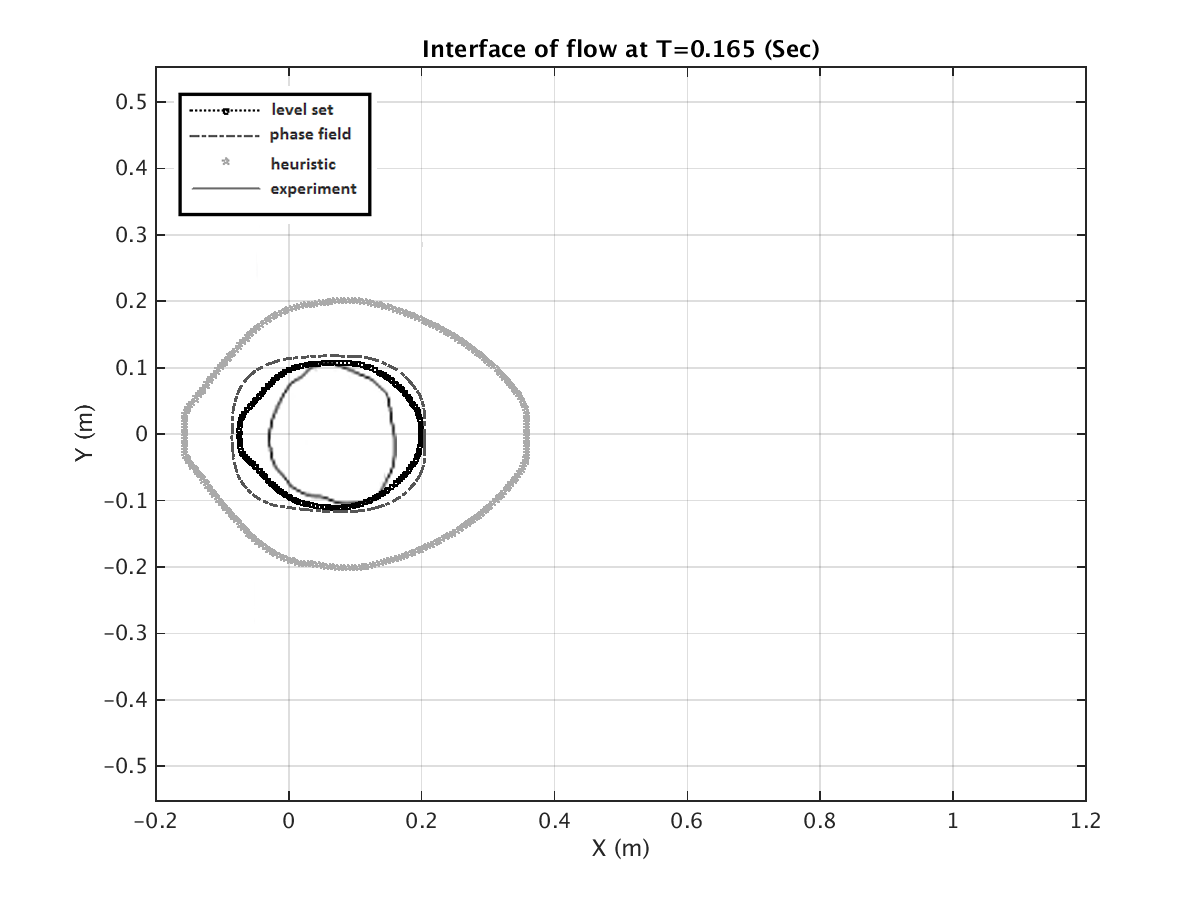
\includegraphics[width=1\textwidth]{IMAGES/interface165exp.png}
                \subcaption{T=0.165 sec}
                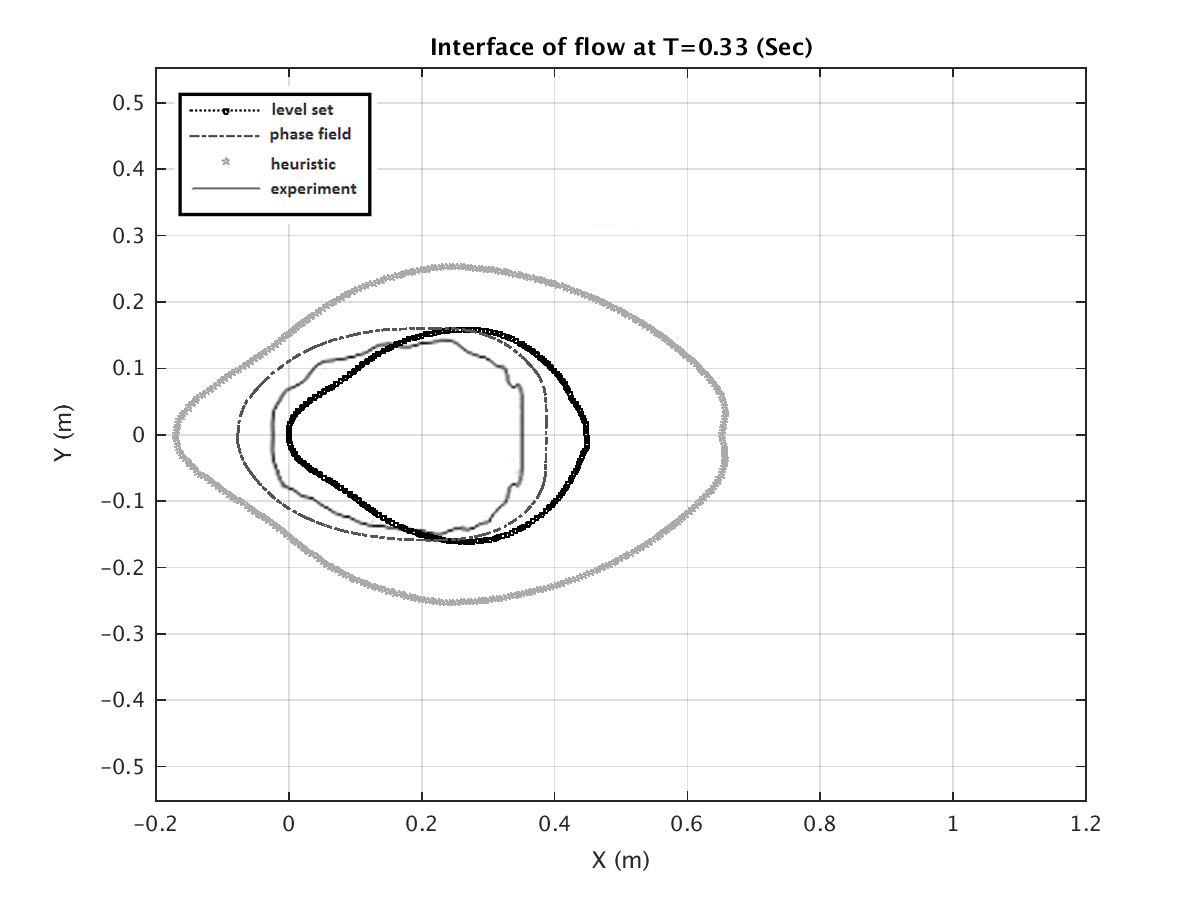
\includegraphics[width=1\textwidth]{IMAGES/interface330exp.png}
                \subcaption{T=0.33 sec}
        \end{minipage}
        %   \hfill
        \begin{minipage}[b]{.48 \linewidth}
                \centering
                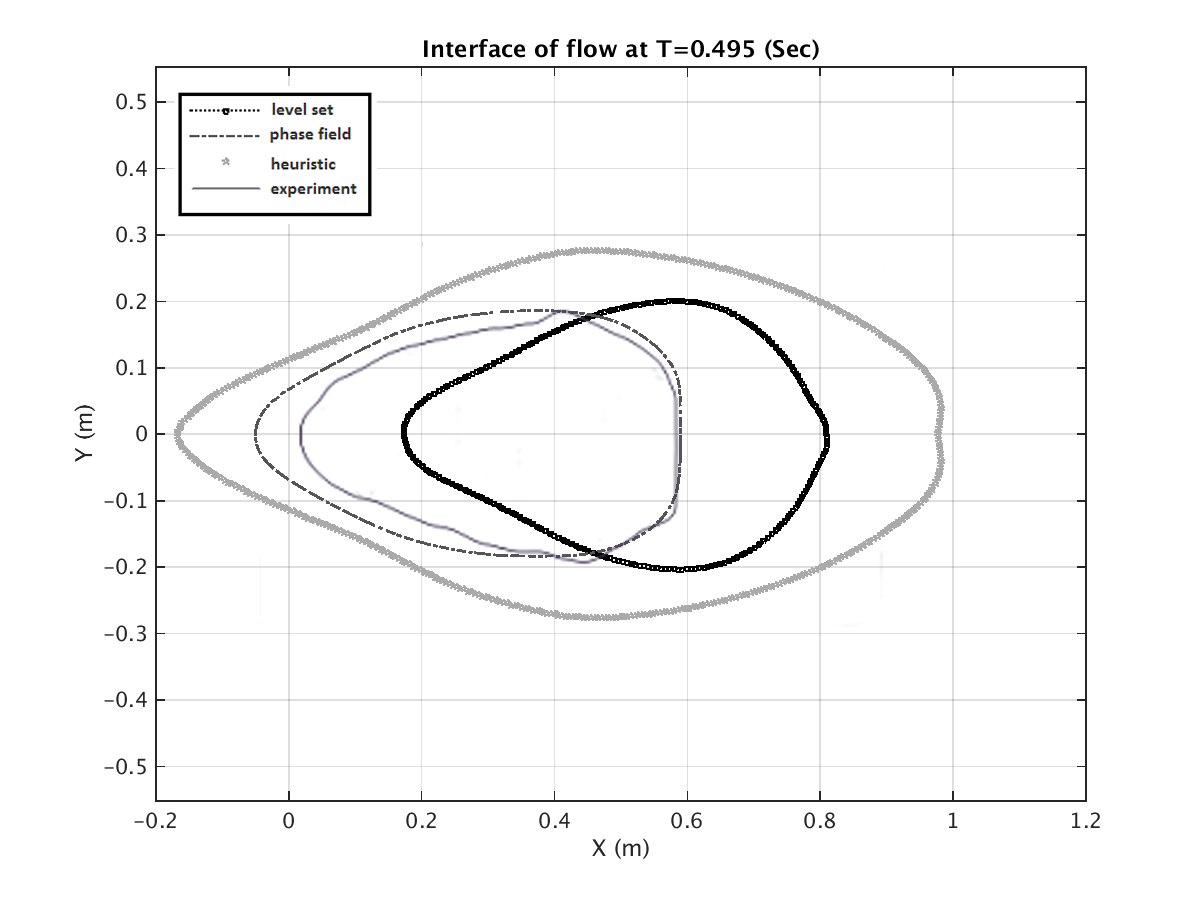
\includegraphics[width=1\textwidth]{IMAGES/interface495exp.png}
                \subcaption{T=0.495 sec}
                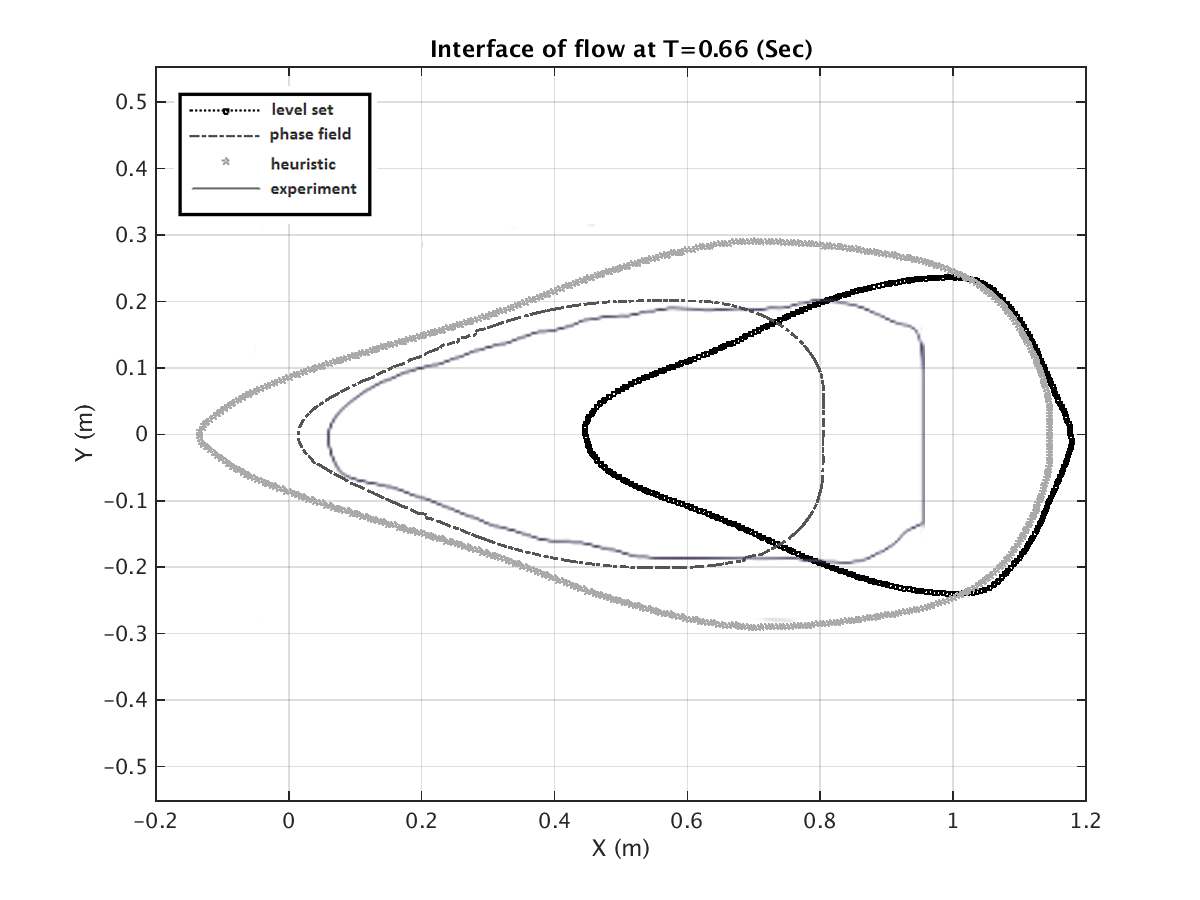
\includegraphics[width=1\textwidth]{IMAGES/interface660exp.png}
                \subcaption{T=0.66 sec}
        \end{minipage}
        \caption{Pile height contour and interface location at different time steps}
        \label{odinary}
\end{figure}
\subsubsection{Comparison}
For quantitative comparison of the results, we compared different schemes on three measurable quantities. The first measure is the extent of pile in X direction, the second one the extent of pile in Y direction, and the last one is the area of pile.
\begin{figure}[H]
        \begin{minipage}[b]{.48\linewidth}
                \centering
                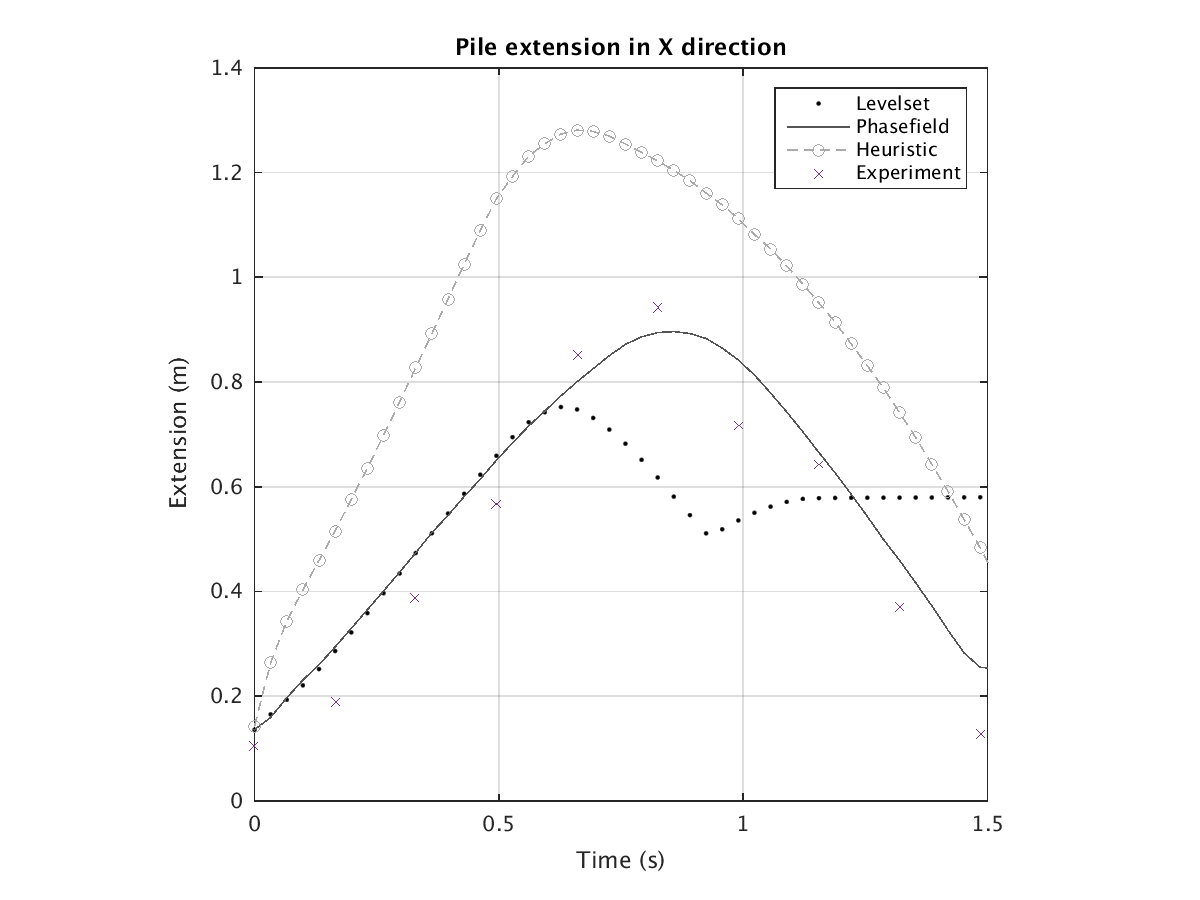
\includegraphics[scale=0.48]{IMAGES/xextend.png}
                \subcaption{Extension of pile in X direction}
                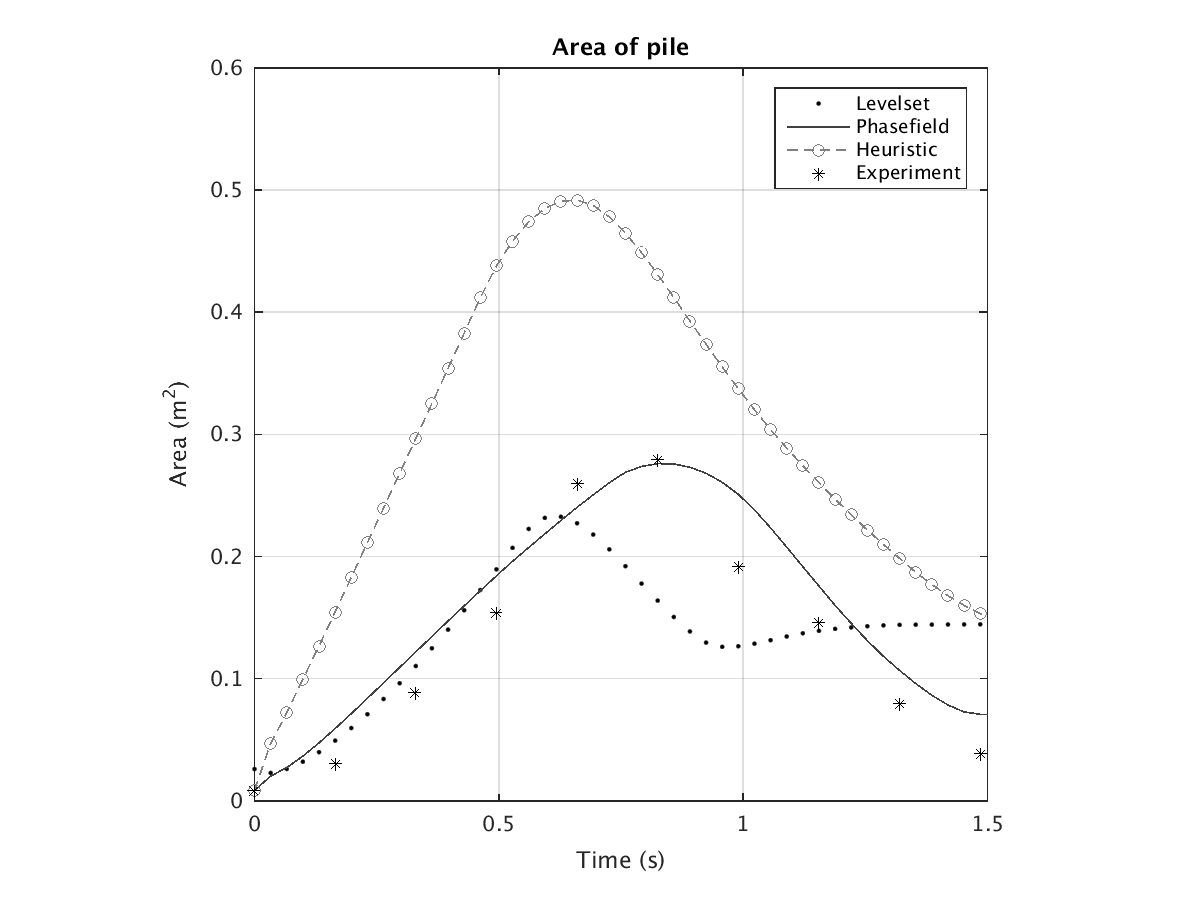
\includegraphics[scale=0.48]{IMAGES/area.png}
                \subcaption{Area of pile}
        \end{minipage}
        %   \hfill
        \begin{minipage}[b]{.48 \linewidth}
                \centering
                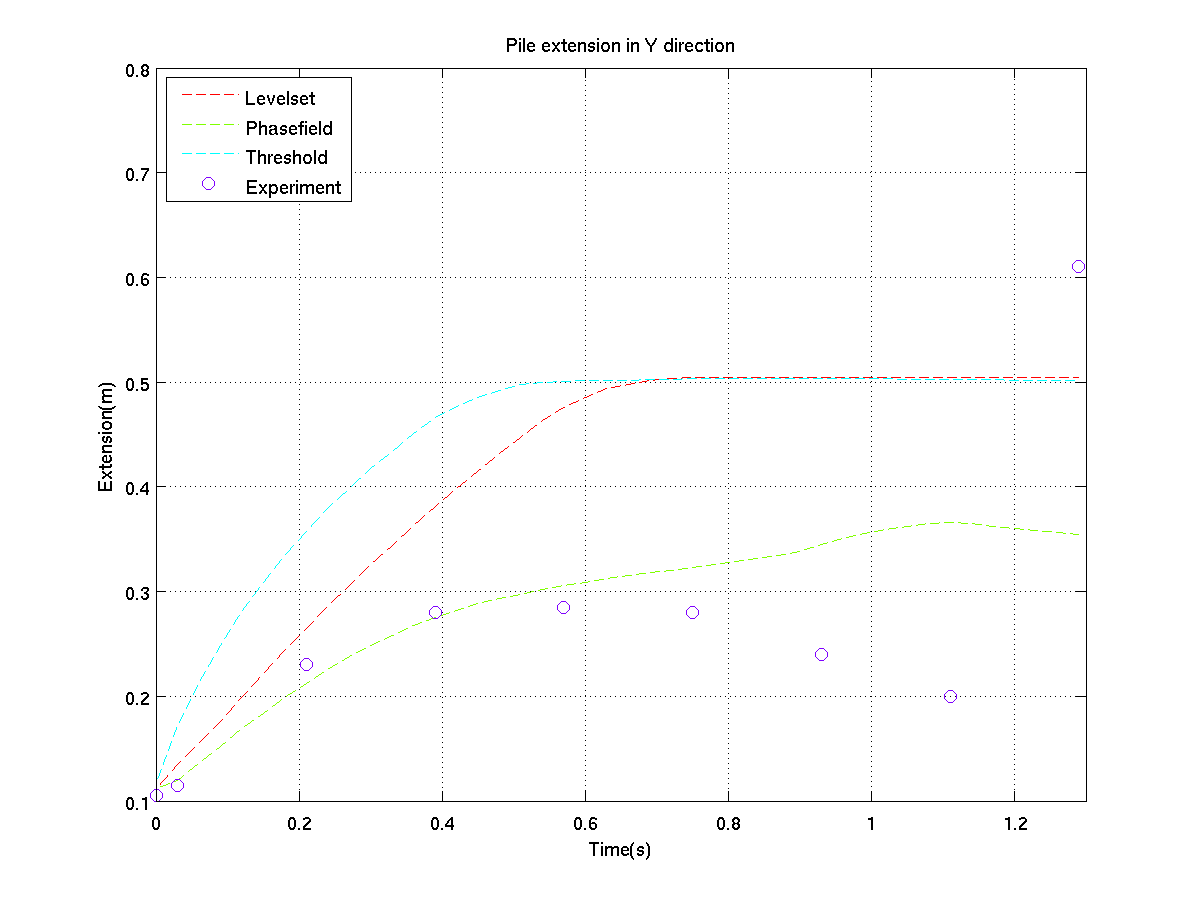
\includegraphics[scale=0.48]{IMAGES/yextend.png}
                \subcaption{Extension of pile in Y direction}
                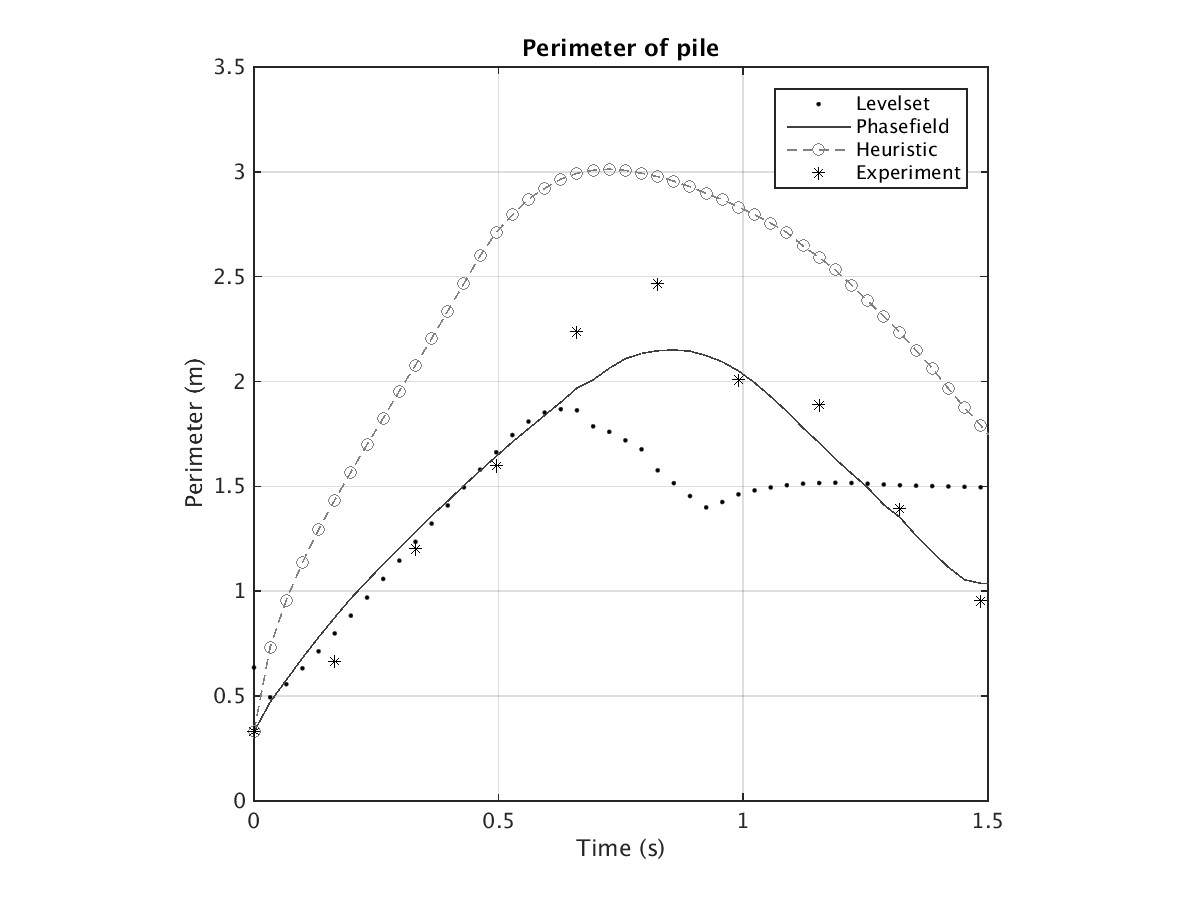
\includegraphics[scale=0.48]{IMAGES/perimeter.png}
                \subcaption{Perimeter of pile}
        \end{minipage}
        \caption{Comparison of the methods for flow on inclined plane}
        \label{compinc}
\end{figure}
% \end{figure}
\subsection{Colima Volcano}
%{\huge keith wants the result of Atentique }\\
In this section, we verify our different interface capturing methods with a field data of an eruption of Colima volcano. 
Colima volcano in Mexico is one of the most active volcanoes in North America, and this eruption happened on 16-17 April 1991 \cite{Charbonnier2008}. 
\begin{center}
        \begin{tabular}{|l|c|}
%               \hline
%               Colima volcano input parameters
                \hline
                Location of pile in X     & 644900.0 \\
                \hline
                Location of pile in Y     & 2157700.0 \\
                \hline
                Maximum pile height       & 40 m \\
                \hline
                Major extent of the pile  & 112.68 m \\
                \hline
                Minor extent of the pile  & 113 m \\
                \hline           
                Bed friction angle        & $37^o$ \\
                \hline
                Internal friction angle  & $20^o$ \\
                \hline
        \end{tabular}
\end{center}
The topography of Colima volcano is such that small changes the initial location of the pile leads to a completely different 
path of flow, so a good performance of any of the interface capturing methods for this case promises a reliable method for other volcanoes.
To be able to compare our results with the outline of deposit of flow, we record the history of all points with the finest 
resolution of the mesh during the simulation to check the points that are placed exactly on the boundary of the flow. 
As a definition boundary here means that the points that the flow passed from them, but has not passed one of their neighbors 
in different directions. For phase field and level set just with recording the maximum absolute value of $ \phi $ we can find 
these points by plotting $\phi=0$, this contour produces deposit line of flow during the time. For the heuristic method we 
recorded the minimum of the pile height during time and plotted the contour of $ h = h_{scale} \times GEOFLOW \_ TINY$, where 
$ h_{scale} =Volume^\frac{1}{3} $.
% \text{Height_Scale}
% \text{Height_Scale}
The resolution of the digital elevation model (DEM) of Colima volcano that here we used is 5 meter which is the finest DEM 
that we have ever used for this volcano.
The outline of this eruption is available in \cite{NamikawaPhD}, we used the method that is described in \cite{NamikawaPhD} to 
extract the skeleton line of the flow to be able to compare the results quantitatively. The procedure of the extraction of the 
skeleton line is shown in the following pictures. 
\begin{figure}
        \centering
        \begin{subfigure}[b]{0.45\textwidth}
                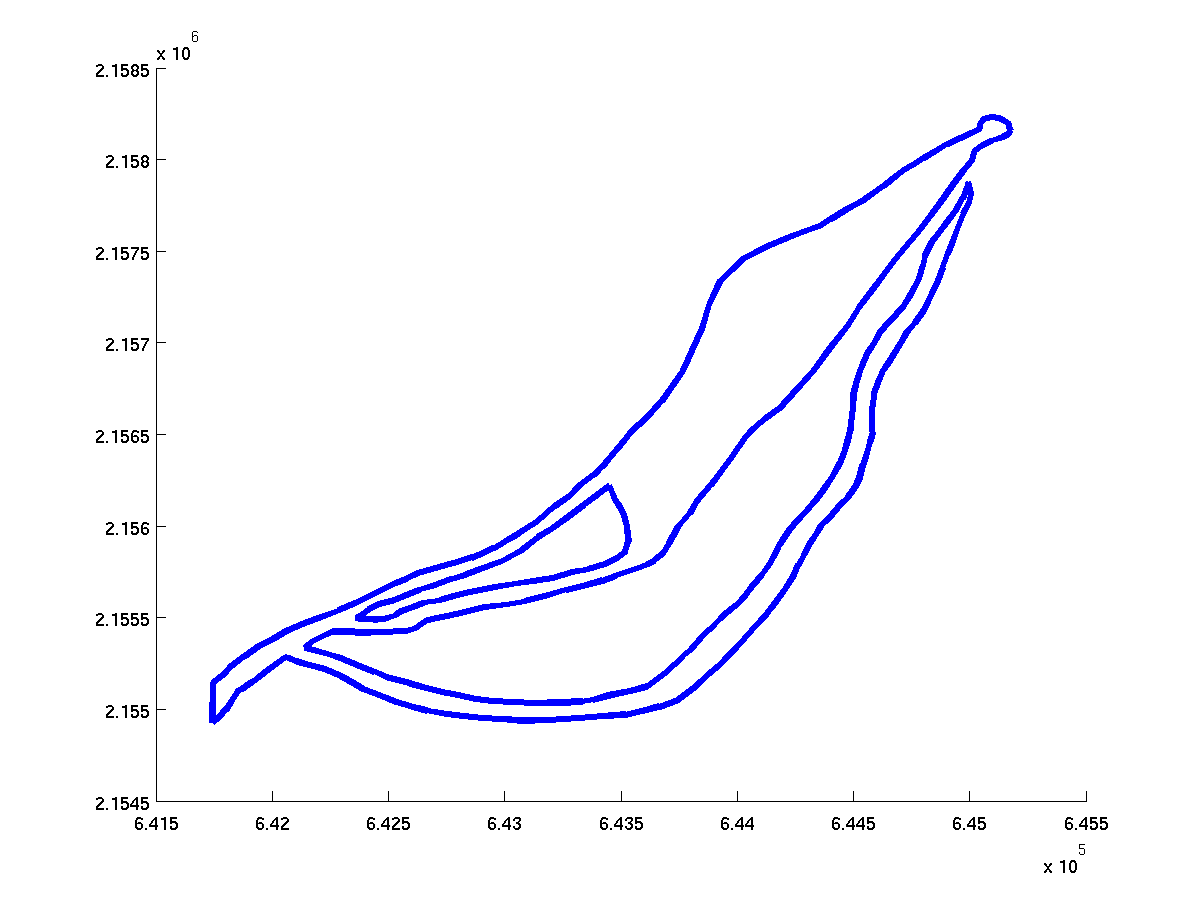
\includegraphics[width=\textwidth]{IMAGES/pics/outline.png}
                \caption{Outline of flow from field data}
                \label{fig:Outline}
        \end{subfigure}%
        \begin{subfigure}[b]{0.45\textwidth}
                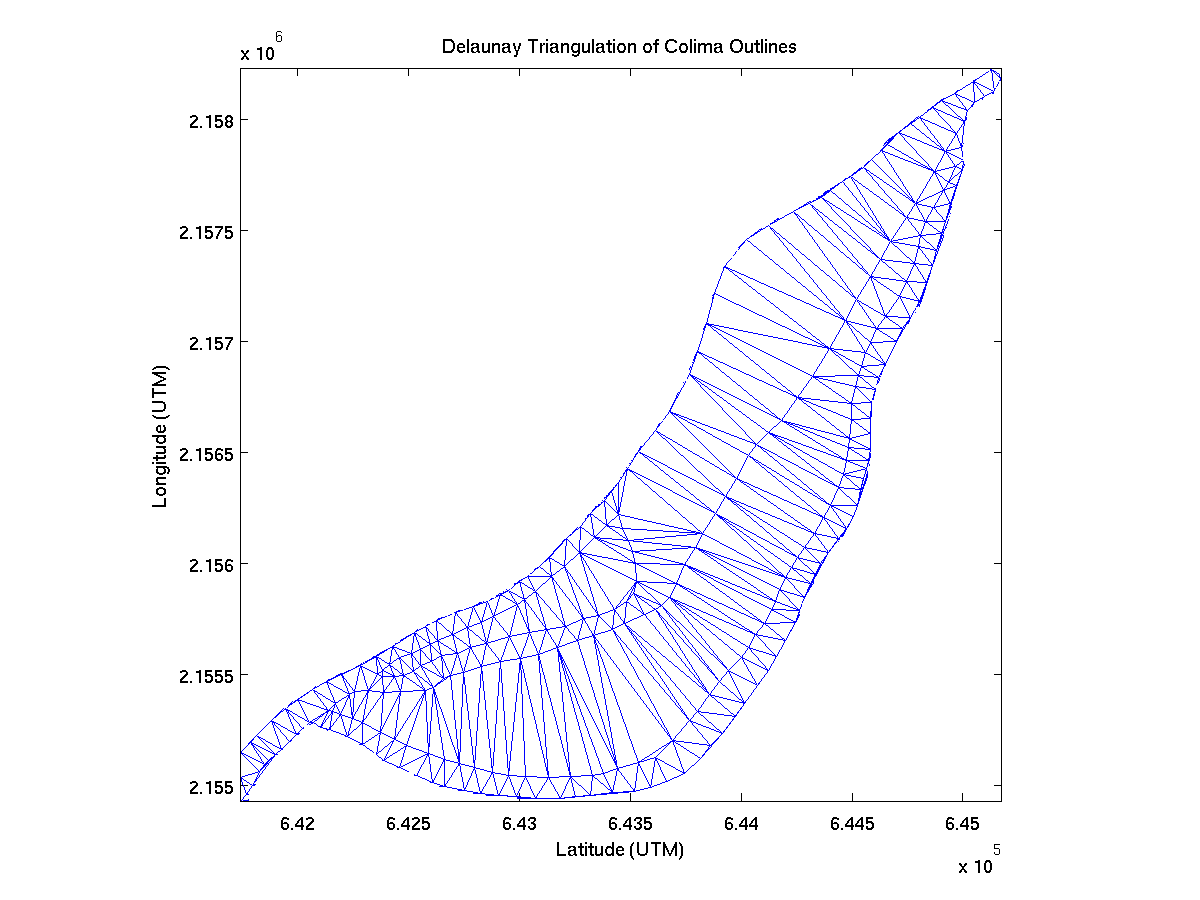
\includegraphics[width=\textwidth]{IMAGES/pics/Delaunay_Triangulation_of_Colima_clean.png}
                \caption{Delaunay triangulation based on the outline of the flow}
                \label{fig:Delaunay}
        \end{subfigure}\\
        \begin{subfigure}[b]{0.45\textwidth}
                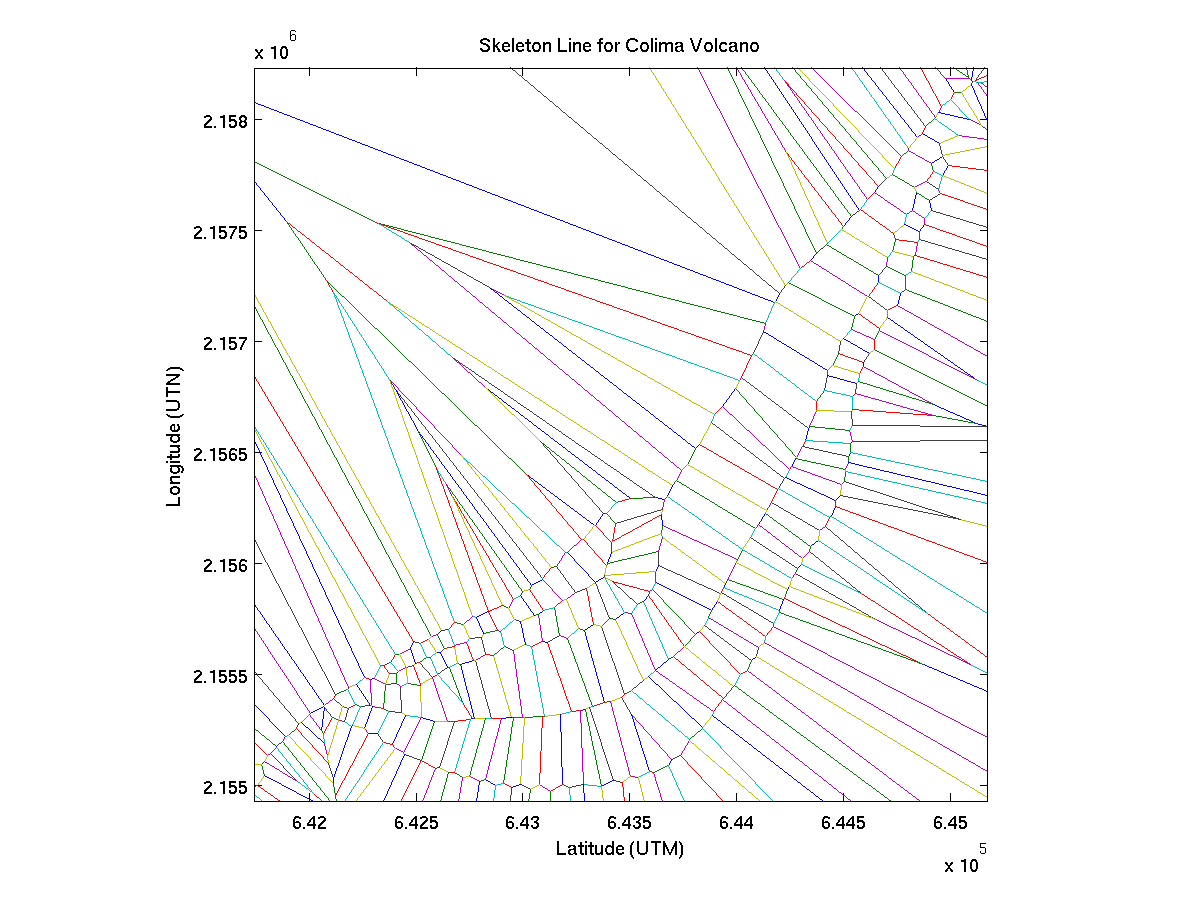
\includegraphics[width=\textwidth]{IMAGES/pics/Skeleton_line.png}
                \caption{Finding the middle of the edges of the triangles that connects the outline of the flow}
                \label{fig:veroni}
        \end{subfigure}
        \begin{subfigure}[b]{0.45\textwidth}
                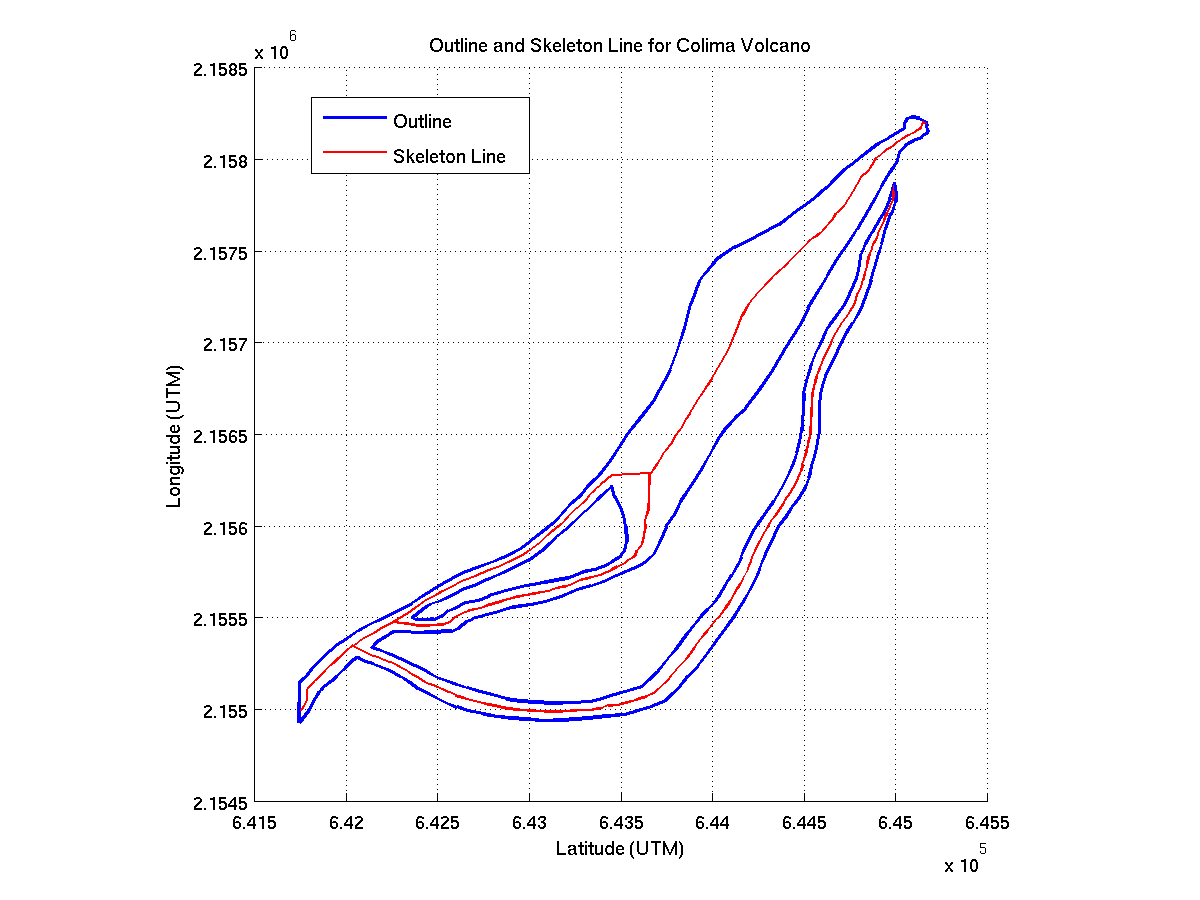
\includegraphics[width=\textwidth]{IMAGES/pics/Outline_Skeleton_line.png}
                \caption{Connecting the middle verticals that are inside of the outline of the flow, in this picture the
                outline of the flow (blue line) and the skeleton line of the flow (red line) can be seen}
                \label{fig:skeleton}
        \end{subfigure}
                
        \caption{In this set of pictures the steps that have to be taken for finding the outline of the flow is displayed 
        respectively}\label{fig:skeleton_line_proc}
\end{figure}
%\newpage
After finding the skeleton line, we mapped the outline of the flow and the skeleton line on the Colima volcano 
using Keyhole Markup Language (KML) and Google earth application \ref{skel_outline}. In figure \ref{Colimapic} the result of each methods and their comparison can be seen. 
\begin{figure}[H]
\centerline{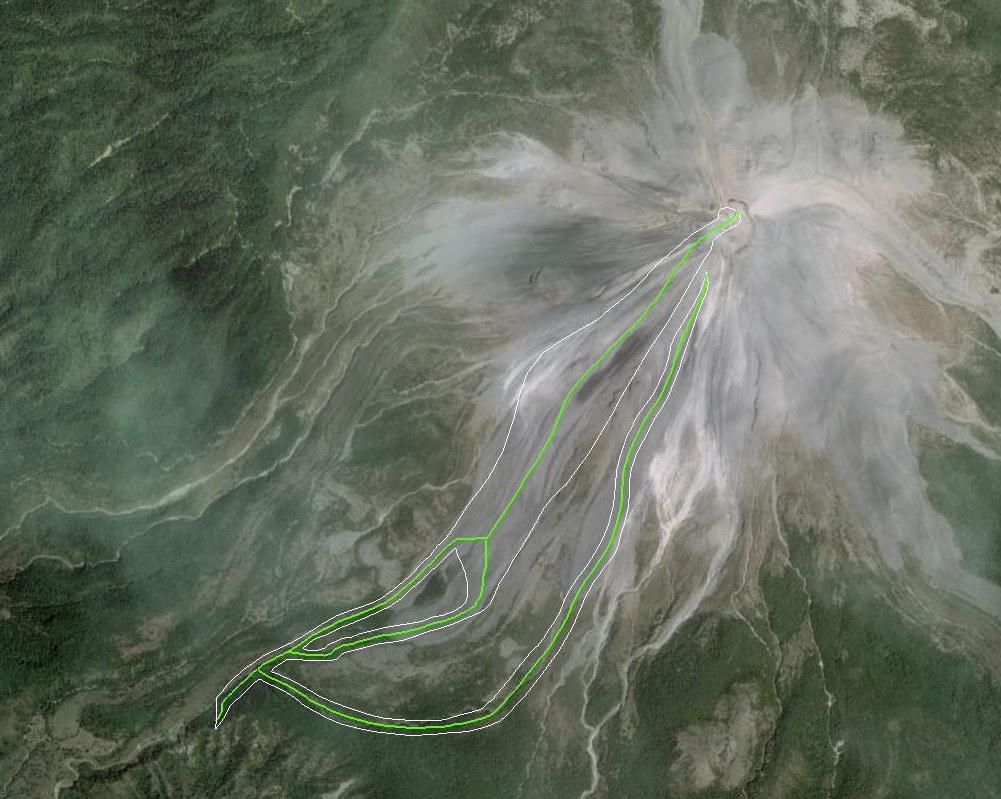
\includegraphics[width=.35\textwidth]{IMAGES/skeleton_outline1.jpg}}
\caption{Skeleton line (white line) and outline of the deposit of eruption 1991 (green line)}
\label{skel_outline}
\end{figure}
\begin{figure}[H]
        \begin{minipage}[b]{.48\linewidth}
        \centering
                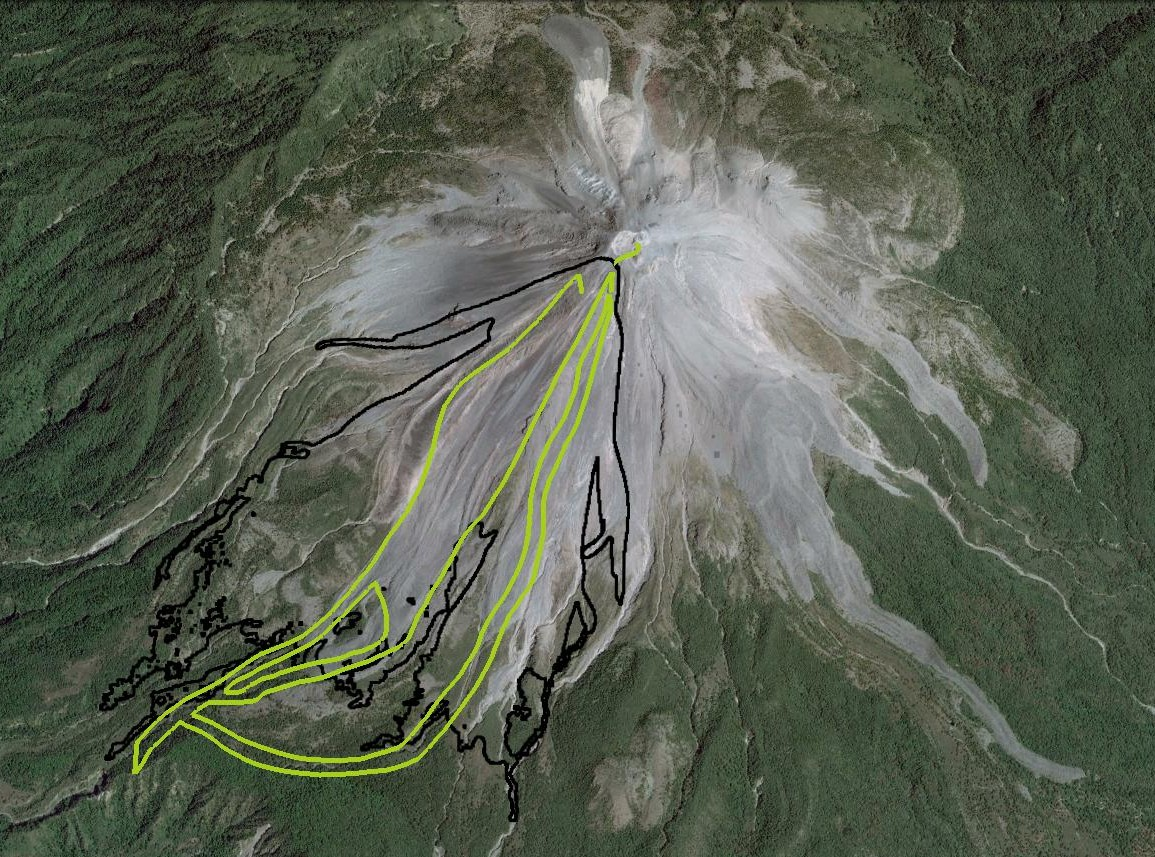
\includegraphics[width=.95\textwidth]{IMAGES/tiny1.jpg}
                \subcaption{Outline from Heuristic Method}
                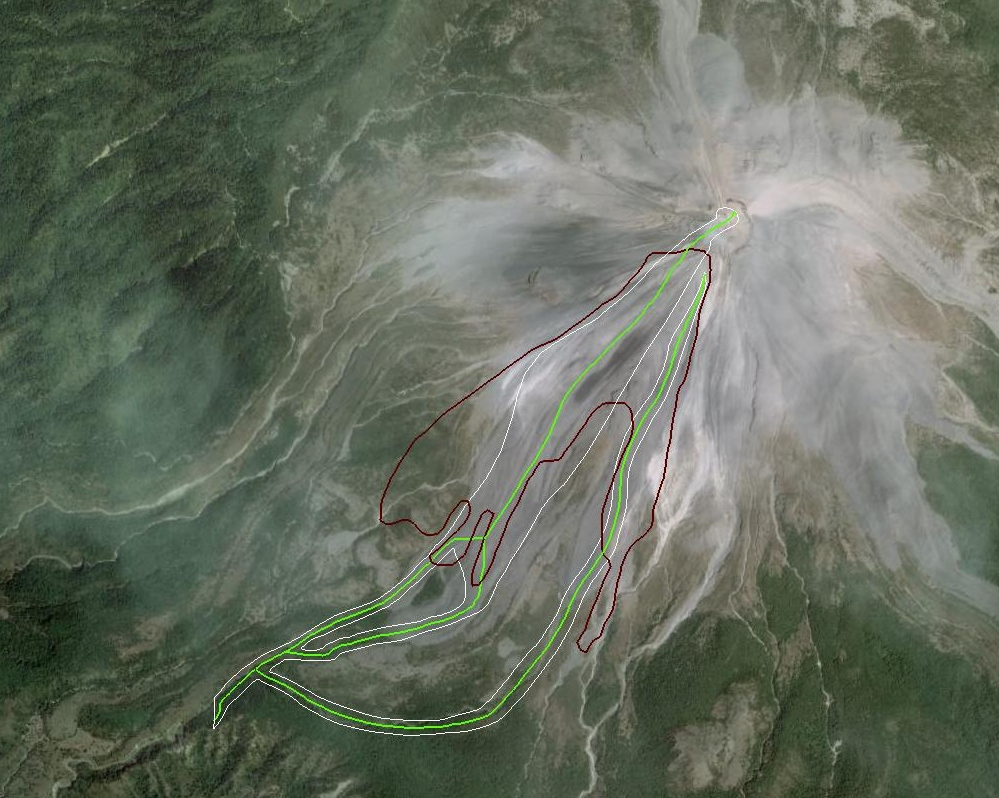
\includegraphics[width=.95\textwidth]{IMAGES/levelset1.jpg}
                \subcaption{Outline from Level set Method}
        \end{minipage}
        %   \hfill
        \begin{minipage}[b]{.48 \linewidth}
                \centering
                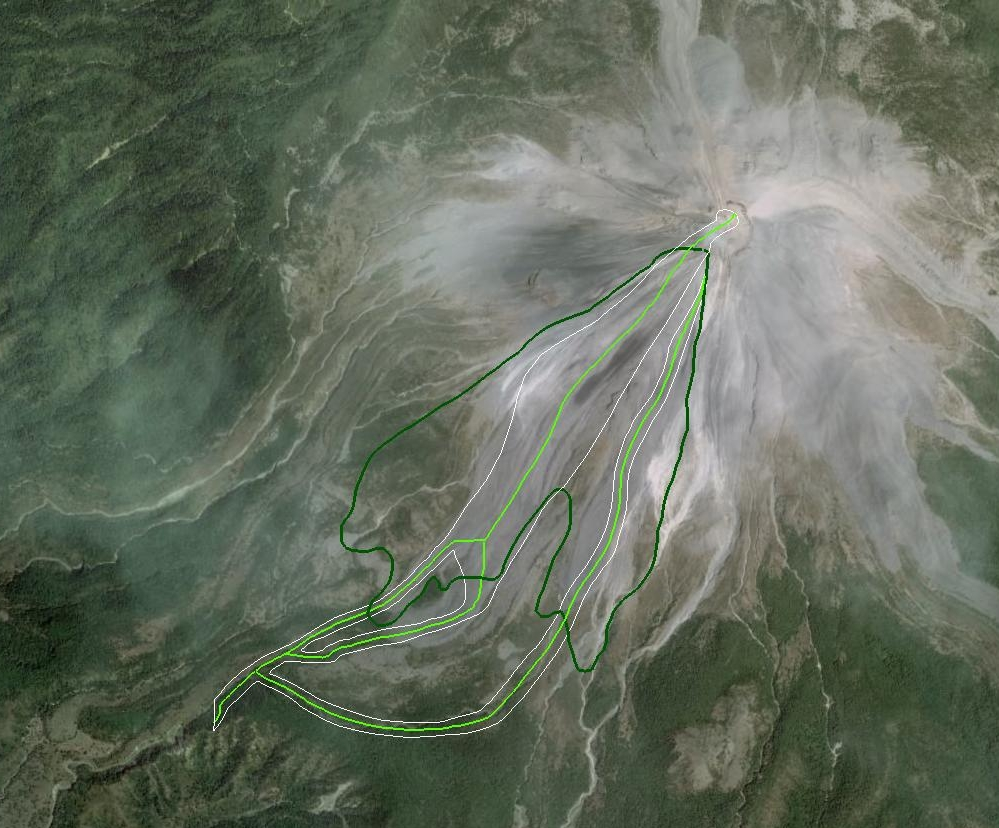
\includegraphics[width=.95\textwidth]{IMAGES/phasefield1.jpg}
                \subcaption{Outline from Phase field Method}
                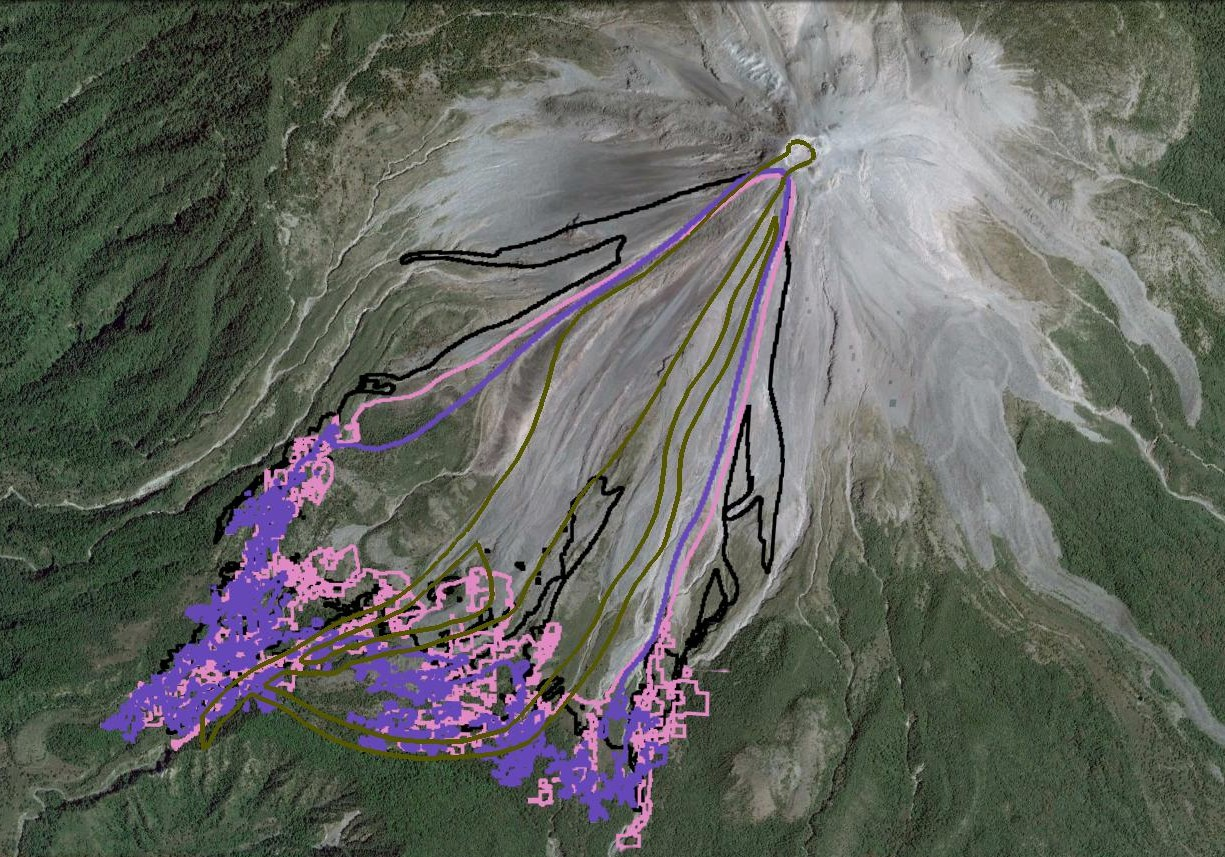
\includegraphics[width=.95\textwidth]{IMAGES/comparison1.jpg}
                \subcaption{Comparison of all three methods}
        \end{minipage}
        \caption{Comparison of the obtained outline of flow from Heuristic, Level set, and Phase field methods for Colima Volcano}
        \label{Colimapic}
\end{figure}
%\begin{figure}[H]
%\centerline{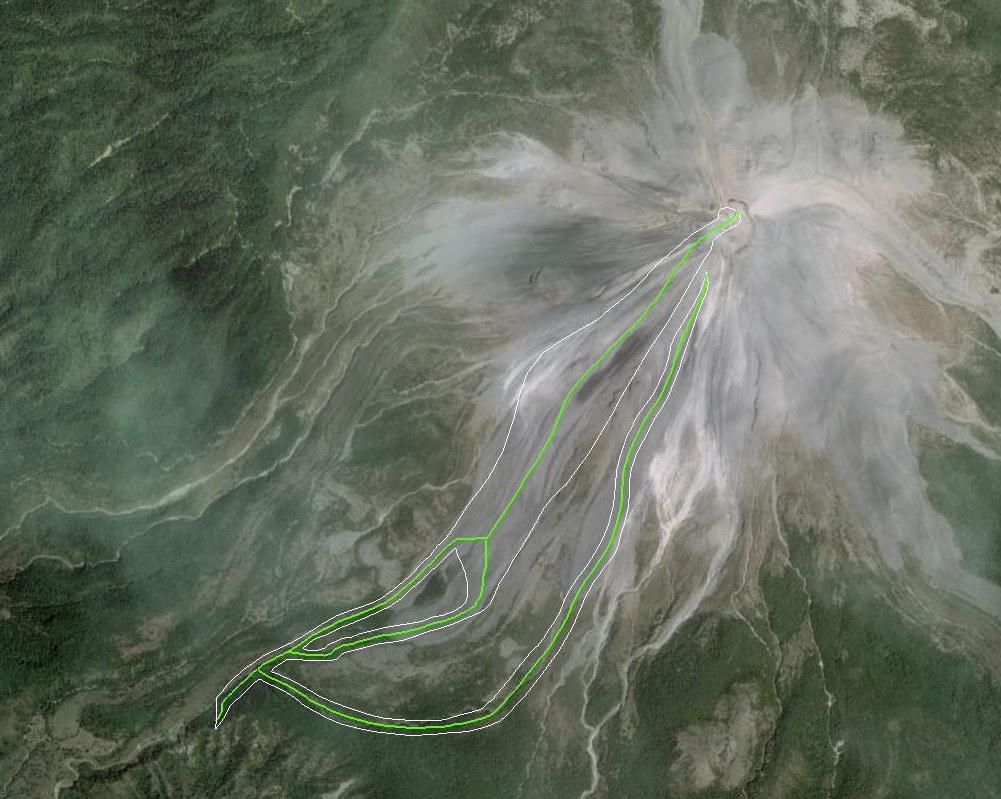
\includegraphics[width=.5\textwidth]{IMAGES/skeleton_outline1.jpg}}
%\caption{Skeleton line (white line) and outline of the deposit of eruption 1991 (yellow line)}
%\label{skel_outline}
%\end{figure}
%
%\begin{figure}[H]
%\centerline{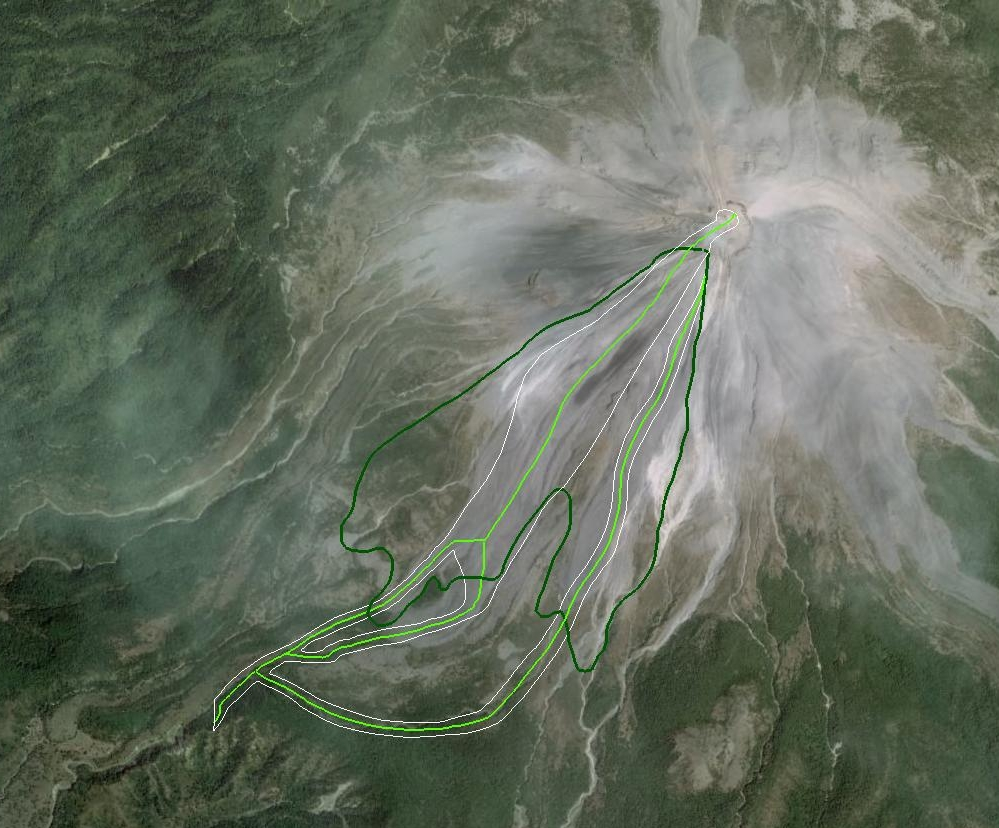
\includegraphics[width=.5\textwidth]{IMAGES/phasefield1.jpg}}
%\caption{}
%\label{phasecolima}
%\end{figure}
%
%\begin{figure}[H]
%\centerline{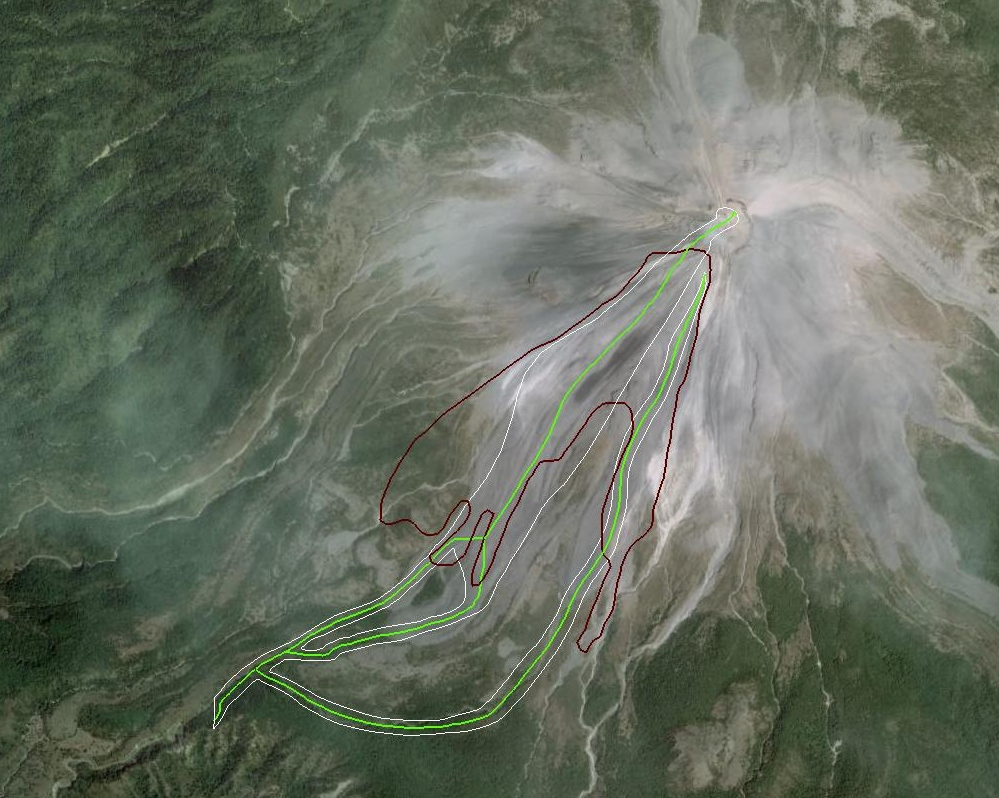
\includegraphics[width=.5\textwidth]{IMAGES/levelset1.jpg}}
%\caption{Skeleton line (white line) and outline of the deposit of eruption 1991 (yellow line)}
%\label{level_colima}
%\end{figure}
% 
% \begin{figure}[H]
% \centerline{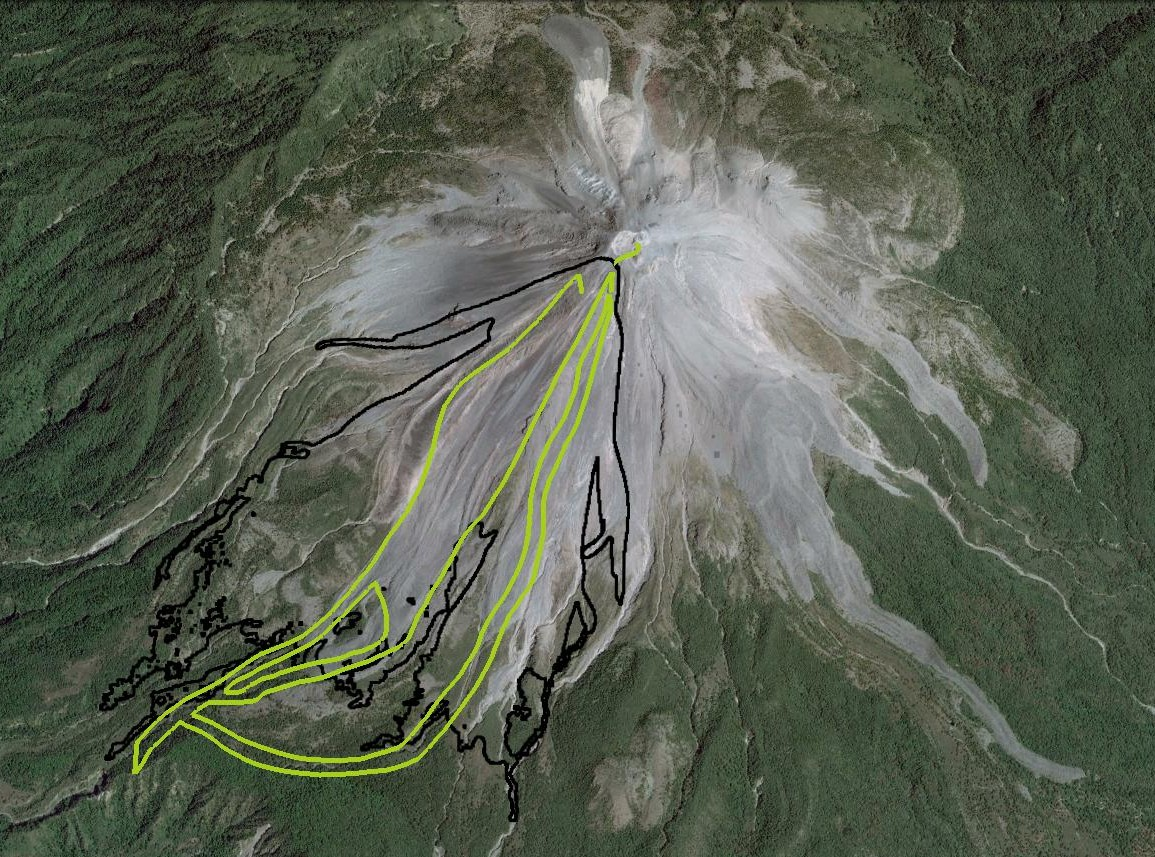
\includegraphics[width=.5\textwidth]{IMAGES/tiny1.jpg}}
% \caption{Skeleton line (white line) and outline of the deposit of erution 1991 (yellow line)}
% \label{tiny_colima}
% \end{figure}
% 
% \begin{figure}[H]
% \centerline{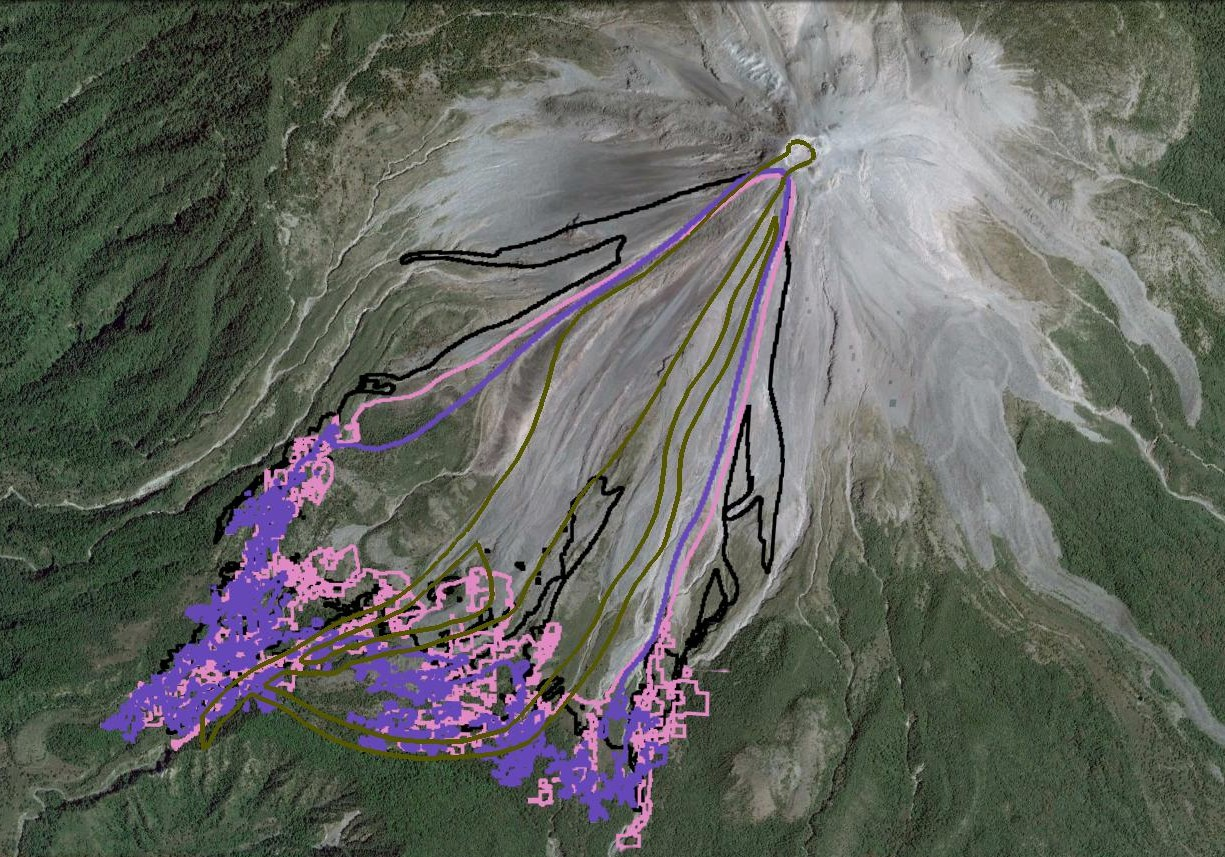
\includegraphics[width=.5\textwidth]{IMAGES/comparison1.jpg}}
% \caption{Skeleton line (white line) and outline of the deposit of erution 1991 (yellow line)}
% \label{compfig}
% \end{figure}
\section{Conclusions} \label{conclusions}
The numerical solution of the Savage-Hutter (and similar 
``shallow-water'') equations have historically been plagued by 
several interrelated numerical difficulties which are collectively characterized by a non-physically thin-layer extending large distances from the realistic main body of the flow. 
In the best case, this ``thin-layer problem'' means a ``no flow'' boundary line must be arbitrarily drawn at some given depth contour.  In 
the worst case, it can cause severe numerical instability that 
prevents any simulation of a particular event.
In this paper, we 
have described some features of the thin-layer problem,
some underlying causes that are common to virtually all numerical 
solution methodologies.  Moreover, we presented a heuristic method and compared 
two interface capturing approaches that 
mitigate this problem by addressing its root causes. In heuristic method we used a threshold to distinguish between wet and dry areas, and in the level set and phase field methods we solved a 
transport equation that implicitly represents the interface of the flow. Then we used the result of previous step for mesh refinement in all of the three solvers to control the thin layer problem and other related problems. Moreover in the heuristic approach we also used this result for interface reconstruction  and adjusting the flux. 
We implemented these thin-layer control strategies in TITAN2D, our high 
performance finite volume solver of the depth-averaged granular 
flow equations.  Numerical simulations were performed for 
geophysical mass flows at two different cases.
To verify the solvers, numerical experiments were conducted for an inclined plate that finally continues horizontally, and Colima volcano. For the first case we verified the numerical results 
with experimental results, and for the second case we compared the results with field data. These analysis showed that with all of the approaches,
which not only prevented the loss of numerical stability but also demonstrated behavior that is consistent with expectations.
%
%As the second case, we tested our solvers on Colima volcano, which is an active volcano 
%in Mexico, was selected on the basis that the DEM had provoked 
%thin-layer numerical difficulties from an earlier version of TITAN2D, 
%and that a campanologist familiar with the location had selectively 
%tuned TITAN2D's few input parameters and also computational and 
%post-processing thresholds to produce results that closely matched 
%reality for that location. The new version of TITAN2D, which implemented
%our thin-layer control strategy, automatically (i.e. without 
%tuning) reproduced a flow outline that had even greater agreement 
%with the historical data. 
%
%Then the results of these approaches were compared. The result of this comparison showed 
%a very good consistency between these approaches.
% Therefore the phase field method could be used for finding the flow boundary 
% of flow and handle the WD problem. 
On the basis of these very positive results, we concluded that our 
thin-layer control strategy, and interface capturing approach provides sufficient benefit. 
While all of these approaches to thin-layer mitigation was developed in the 
context of TITAN2D's capabilities, much of it should be appropriate 
for use in depth-averaged flow solvers with different numerical 
implementations.
\newpage
\appendix
 
\bibliographystyle{plain}
\bibliography{mybib}
\end{document}
